\documentclass[leqno,12pt]{article}

%=====================================================================
%============================= packages ==============================

\usepackage{amsmath}
\usepackage[utf8]{inputenc} 
\usepackage[T1]{fontenc}
\usepackage[varg]{txfonts}
\usepackage{times}
%\usepackage{microtype}
\usepackage{amssymb}
\usepackage{stmaryrd}
\usepackage{fancyhdr}
\usepackage{natbib}
\usepackage[normalem]{ulem}
\usepackage{examples-slim}
\usepackage{color}
\usepackage{xcolor}
\usepackage{graphicx}
\usepackage{float}
\usepackage{booktabs}
\usepackage{colortbl}
\usepackage{qtree}
\usepackage{ifthen}
\usepackage{caption}
\usepackage{subcaption}
\usepackage{multirow}
\definecolor{black}{HTML}{000000}
\usepackage[colorlinks, linkcolor=black, urlcolor=black, citecolor=black]{hyperref}

% Good colors for colorblind readers (apparently):
\definecolor{cbgreen}{HTML}{1B9E77}
\definecolor{cborange}{HTML}{D95F02}
\definecolor{cbpurple}{HTML}{7570B3}

\bibpunct[; ]{(}{)}{;}{a}{}{,}  % natbib citation style

\defcitealias{ChierchiaFoxSpector08}{CFS}
\newcommand{\CFS}{\citetalias{ChierchiaFoxSpector08}}
\defcitealias{Geurts:Pouscoulous:2009}{G\&S}
\newcommand{\GP}{\citetalias{Geurts:Pouscoulous:2009}}

%=====================================================================
%========================= cross-references ==========================

% Flexible sec/fig/tbl/def cross-refs.
\newcommand{\Secref}[1]{Section~\ref{#1}}
\newcommand{\secref}[1]{section~\ref{#1}}
\newcommand{\dashsecref}[2]{sections~\ref{#1}--\ref{#2}}

% \newcommand{\Defref}[1]{Def.~\ref{#1}}
% \newcommand{\defref}[1]{def.~\ref{#1}}
% \newcommand{\Defrefc}[2]{\Defref{#1}, clause~\ref{#2}}
% \newcommand{\defrefc}[2]{\defref{#1}, clause~\ref{#2}}

\newcommand{\Figref}[1]{Figure~\ref{#1}}
\newcommand{\figref}[1]{figure~\ref{#1}}
\newcommand{\dashfigref}[2]{figures~\ref{#1}--\ref{#2}}
\newcommand{\Tabref}[1]{Table~\ref{#1}}
\newcommand{\tabref}[1]{table~\ref{#1}}

\newcommand{\Appendixref}[1]{Appendix~\ref{#1}}
\newcommand{\appendixref}[1]{appendix~\ref{#1}}

% Examples:
\newcommand{\eg}[1]{(\ref{#1})}
\newcommand{\subeg}[2]{(\ref{#1}\ref{#2})}
\newcommand{\dblsubeg}[3]{(\ref{#1}\ref{#2},~\ref{#3})}
\newcommand{\dashsubeg}[3]{(\ref{#1}\ref{#2}--\ref{#3})}

% In-text citations
\newcommand{\posscitet}[1]{\citeauthor{#1}'s~(\citeyear{#1})}
\newcommand{\sposscitet}[1]{\citeauthor{#1}'~(\citeyear{#1})}
\newcommand{\possciteauthor}[1]{\citeauthor{#1}'s}
\newcommand{\spossciteauthor}[1]{\citeauthor{#1}'}
\newcommand{\pgposscitet}[2]{\citeauthor{#1}'s~(\citeyear{#1}:~#2)}
\newcommand{\secposscitet}[2]{\citeauthor{#1}'s~(\citeyear{#1}:~$\S$#2)}
\newcommand{\pgcitealt}[2]{\citealt{#1}:~#2}
\newcommand{\seccitealt}[2]{\citealt{#1}:~$\S$#2}
\newcommand{\pgcitep}[2]{(\citealt{#1}:~#2)}
\newcommand{\seccitep}[2]{(\citealt{#1}:~$\S$#2)}
\newcommand{\pgcitet}[2]{\citeauthor{#1}~(\citeyear{#1}:~#2)}
\newcommand{\seccitet}[2]{\citeauthor{#1}~(\citeyear{#1}:~$\S$#2)}

%=====================================================================
%============================ text styles ============================

\newcommand{\word}[1]{\emph{#1}}
\newcommand{\tech}[1]{\textbf{#1}}
\newcommand{\highlight}[1]{\uline{#1}}

%\newcommand{\magentahighlighter}[1]{\colorbox{magenta}{#1}}
\newcommand{\magentahighlighter}[1]{\textcolor{magenta}{#1}}
% Gray table cell:
\newcommand{\graycell}[1]{{\cellcolor[gray]{.8}#1}}

%=====================================================================
%=============================== models ==============================

\newcommand{\set}[1]{\ensuremath{\left\{ #1 \right\}}}
\newcommand{\True}{\texttt{T}}
\newcommand{\False}{\texttt{F}}
\newcommand{\entails}{\sqsubseteq}
\newcommand{\evee}{\mathbin{\overline{\vee}}}
\newcommand{\tuple}[1]{\langle #1 \rangle}

\newcommand{\Reals}{\mathbb{R}}
\newcommand{\given}{\mid}
\newcommand{\Indicator}{\mathbb{I}}

\newcommand{\sem}[1]{\ensuremath{\llbracket#1\rrbracket}}
\newcommand{\States}{W}
\newcommand{\state}{w}
\newcommand{\Lex}{\mathcal{L}}
\newcommand{\LexSet}{\mathbf{L}}
\newcommand{\Messages}{M}
\newcommand{\Refinable}{\textit{Refinable}}
\newcommand{\msg}{m}
\newcommand{\Costs}{C}
\newcommand{\StatePrior}{P}
\newcommand{\LexPrior}{P_{\LexSet}}

\newcommand{\listenerZero}{l_{0}}
\newcommand{\speakerOne}{s_{1}}
%\newcommand{\listenerOne}{l_{1}}
\newcommand{\UncertaintyListener}[1][]{L_{#1}}
\newcommand{\UncertaintySpeaker}[1]{S\negthinspace_{#1}}

\newcommand{\nullmsg}{\mathbf{0}}

\newcommand{\ALT}{\emph{ALT}}
\newcommand{\OALT}{\mathop{O\negthinspace_{\ALT}}}

\newcommand{\Grammar}{\mathcal{G}}
\newcommand{\refine}{\ensuremath{R}}
\newcommand{\Refine}[1][c]{\mathcal{R}_{#1}}

\newcommand{\world}[1]{\texttt{#1}}
\newcommand{\Worlds}{W}
\newcommand{\Domain}{D}

\newcommand{\Likert}{\emph{Likert}}
\newcommand{\target}[2]{`\word{#1}\ldots\word{#2}'}

%=====================================================================
%============================ annotations ============================

\newcommand{\marginnote}[1]{\marginpar[\color{blue}\raggedright\tiny
  #1]{\color{blue}\raggedright\scriptsize #1}}
\newcommand{\Rogersmarginnote}[1]{\marginpar[\color{magenta}\raggedright\tiny #1]{\color{magenta}\raggedright\scriptsize #1}}

\newcommand{\todo}[1]{\marginpar[\color{red}\raggedright\scriptsize #1]{\color{red}\raggedright\scriptsize TODO: #1}}


\newcommand{\mynote}[1]{{\color{red}#1}}

%=====================================================================
%============================== grammar ==============================

\newcommand{\playera}{\texttt{a}}     
\newcommand{\playerb}{\texttt{b}}     
\newcommand{\playerc}{\texttt{c}}
\newcommand{\Vt}{V$_{\text{T}}$}
\newcommand{\Vi}{V$_{\text{I}}$}

% For writing grammar definitions:
\newcommand{\gsem}[1]{\sem{\text{#1}}}

% Attempt to simplify quantifier meaning code:
\newcommand{\genericquantifier}[3][]{%
  \ifthenelse{\equal{#1}{cardinality}}%
  {$\set{\tuple{w, X, Y} : |\set{x : \tuple{w,x} \in X} #2 \set{y : \tuple{w,y} \in Y}| #3}$}
  {$\set{\tuple{w, X, Y} :  \set{x : \tuple{w,x} \in X} #2 \set{y : \tuple{w,y} \in Y}  #3}$}}
  
% Attempt to simplify proper name meaning code:
\newcommand{\genericpn}[1]{\set{\tuple{w, Y} : #1 \in \set{x : \tuple{w,x} \in Y}}}

\newcommand{\scalarlex}[1]{
  \begin{array}[c]{r@{ \ = \ }l}
    \sem{\word{scored}} & \set{#1} \\
    \sem{\word{aced}}   & \set{\tuple{\world{A}, \playera}} \\
    \sem{\word{Player\,B}}      & \text{as in tab.\,\ref{tab:grammar}}
  \end{array}}

\newcommand{\genericscalar}[9]{
  \setlength{\arraycolsep}{2pt}
  \begin{array}[c]{r r r r}
    \toprule
    & \world{N} & \world{S} & \world{A} \\
    \midrule
    \word{B scored} & #1 & #2 & #3 \\
    \word{B aced}   & #4 & #5 & #6 \\
    \nullmsg        & #7 & #8 & #9 \\
    \bottomrule
  \end{array}}

\newcommand{\scalarspeaker}[9]{
  \setlength{\arraycolsep}{2pt}
  \begin{array}[c]{r r r r}
    \toprule
    & \word{B scored} & \word{B aced} & \nullmsg \\
    \midrule
    \world{N}  & #1 & #2 & #3 \\
    \world{S}  & #4 & #5 & #6 \\
    \world{A}  & #7 & #8 & #9 \\
    \bottomrule
  \end{array}}

\usepackage{geometry}

\geometry{
  body={6.5in, 8.5in},
  left=1.0in,
  top=1.0in, 
  bottom=1.0in
}


\hypersetup{
  pdfauthor={Christopher Potts, Daniel Lassiter, Roger Levy, and Michael C. Frank},
  pdftitle={Embedded implicatures as pragmatic inferences under compositional lexical uncertainty},
  pdfsubject={computational pragmatics},
  pdfkeywords={conversational implicatures, scalar implicatures, embedded implicatures, Bayesian pragmatics, experimental pragmatics}
}

\begin{document}

%%%%%%%%%%%%%%%%%%%%%%%%%%%%%%%%%%%%%%%%%%%%%%%%%%%%%%%%%%%%%%%%%%%%%%

\title{Embedded implicatures as pragmatic inferences under compositional lexical uncertainty%
  \thanks{All the data and code used in this paper are available at \url{https://github.com/cgpotts/pypragmods}}}
\author{Christopher Potts, Daniel Lassiter, Roger Levy, and Michael C.~Frank}
\maketitle

%\vspace{-28pt}

\begin{abstract} 
  How do comprehenders reason about pragmatically ambiguous scalar
  terms like \word{some} in complex syntactic contexts?  In Gricean
  theories of conversational implicature, local exhaustification of
  such terms (`only some') is predicted to be impossible if it does
  not strengthen the literal meaning, whereas grammatical accounts of
  implicature predict such construals to be available. Recent
  experimental evidence supports the availability of these local
  enrichments, but the grammatical theories that this evidence
  supports do not provide viable mechanisms for weighting such
  construals against others. We propose a probabilistic model that
  combines previous work on pragmatic inference under `lexical
  uncertainty' with a more detailed model of compositional
  semantics. We show that this model makes accurate predictions about
  new experimental data on embedded implicatures in both non-monotonic
  and downward-entailing semantic contexts. In addition, the model's
  predictions can be improved by the incorporation of neo-Gricean
  hypotheses about lexical alternatives. This work thus contributes to
  a synthesis of grammatical and probabilistic views on pragmatic
  inference.
\end{abstract}

  % How do comprehenders reason about the meaning of pragmatically
  % ambiguous scalar terms like `some' in complex syntactic contexts?
  % In Gricean theories of conversational implicature, comprehenders
  % should consider only the set of global alternatives; but on recent
  % grammatical accounts, locally-enriched meanings should be available
  % as well. Recent experimental evidence supports the availability of
  % these local interpretations, but the grammatical theories that this
  % evidence supports do not provide a viable mechanism for weighting
  % them against other possible interpretations. We propose a
  % probabilistic model that combines previous work on pragmatic
  % inference under `lexical uncertainty' with a more detailed model of
  % compositional semantics. We show that this model makes accurate
  % predictions about new experimental data on embedded implicatures in
  % both non-monotonic and downward-entailing contexts. In addition, the
  % model's predictions can be improved by the incorporation of
  % neo-Gricean hypotheses about lexical alternatives. This work thus
  % contributes to a synthesis of grammatical and probabilistic views on
  % pragmatic inference.

 % \citet{Chemla:Spector:2011} present experimental evidence that
 %  scalar terms like \word{some} in the scope of non-monotonic
 %  quantifiers can be locally enriched to an exhaustified meaning
 %  (`only some'). Such construals are predicted not to occur on Gricean
 %  accounts of conversational implicature, but they are easily within
 %  reach of recent grammar-driven theories like that of
 %  \citealt{ChierchiaFoxSpector08}.  We propose a model that 
 %  embraces the semantic insights of grammar-driven theories, but also offers
 %  a pragmatic explanation for how implicatures arise. The model
 %  straightforwardly synthesizes \posscitet{Bergen:Levy:Goodman:2014}
 %  `lexical uncertainty' model with a full compositional
 %  semantics. After describing it in detail, we present new
 %  experimental evidence that people arrive at locally enrichments, not
 %  just in non-monotonic environments but also (and more
 %  controversially) in downward-entailing ones. We then show not only
 %  that our model generates local enrichments, but also that its
 %  predictions are highly correlated with our experimental data, and
 %  that these predictions can be improved by incorporating neo-Gricean
 %  hypotheses about lexical alternatives.

%\vspace{-16pt}

%%%%%%%%%%%%%%%%%%%%%%%%%%%%%%%%%%%%%%%%%%%%%%%%%%%%%%%%%%%%%%%%%%%%%%

\section{Conversational implicature: Interacting with grammar}\label{sec:introduction}

The linguistic forms that discourse participants exchange with each
other routinely underrepresent the speaker's intended message and
underdetermine the listener's inferences. \citet{Grice75} famously
provided a philosophical framework for understanding the driving
forces behind such pragmatic enrichment. At the heart of this
framework are \tech{conversational implicatures}: social, cognitively
complex meanings that discourse participants create jointly in
interaction.

Perhaps the best-studied examples of language users going beyond the
literal semantics involve weak terms like \word{some} being
strengthened to exclude their communicatively stronger alternatives,
giving rise to construals like `some and not all' or `only some'.
Such inferences are often called \tech{scalar conversational
  implicatures} (SIs), and they are widely assumed to arise via the
same social inferencing mechanisms that are at work in other
implicatures.  However, this assumption has always been
controversial. Even \citeauthor{Grice75} suggested that SIs might be
closer to the grammar than other implicatures (p.~56; see also
\citealt{Levinson00,Sperber95,Bach06}), and recent grammar-driven
accounts are framed in direct opposition to an implicature analysis.
For example, \pgcitet{ChierchiaFoxSpector08}{2316} write, ``the facts
suggest that SIs are not pragmatic in nature but arise, instead, as a
consequence of semantic or syntactic mechanisms''. The ensuing debates
have stimulated new insights, pushing researchers to identify and
evaluate previously unnoticed consequences of the two broad positions.

Much of the debate between Gricean and grammar-driven accounts has
centered around what we informally called \tech{embedded implicatures}
--- cases where a pragmatically enriched interpretation seems to be
incorporated into the compositional semantics. Such readings seem
initially to demand implicature-enriched semantic representations.
However, many of the relevant examples have received straightforward
Gricean accounts in which semantic content and contextual assumptions
interact to yield global implicatures that are meaning-equivalent to
interpretations that would derive from local pragmatic enrichment
\citep{Russell06,Geurts09}. This reduces the power of such examples to
decide in favor of one side or the other.

\citet{Geurts:Pouscoulous:2009} and \citet{Chemla:Spector:2011} study
a wide range of embedded implicatures involving scalar terms in the
scope of quantified phrases. They show that many of these listener
inferences are amenable to Gricean treatments with no need for the
pragmatics to intrude on the semantics. However, they identify a class
of examples that will not admit such a treatment: scalar terms in the
scope of non-monotone quantifiers, as in \word{Exactly one player hit
  some of his shots}. In such cases, the interpretation enriched by an
embedded implicature (\word{\ldots some but not all of his shots})
does not entail the literal meaning, whereas the Gricean analysis of
scalar terms can only strengthen literal
meanings. \citeauthor{Geurts:Pouscoulous:2009}'s experiments fail to
support enrichment in such contexts, whereas
\citeauthor{Chemla:Spector:2011}'s suggest that it is possible.

In this paper, we reproduce the central qualitative result of
\citet{Chemla:Spector:2011} using more naturalistic experimental
stimuli and a more direct method of interpreting participants'
responses. Like \citeauthor{Chemla:Spector:2011}, we find that scalar
terms in non-monotone environments support implicature inferences. We
hope that these results bolster \citeauthor{Chemla:Spector:2011}'s
conclusions and help to address the skeptical reactions of
\citet{geurts-vantiel:2013:scalar}. In our view, this evidence points
to a role for compositional semantics in understanding
implicatures. But pragmatic factors also play a crucial role: even
embedded implicatures arise only with proper contextual support
\citep{Russell06,ChierchiaFoxSpector08,Geurts:2011,Chemla:Spector:2011}.

To describe the complementary roles of grammar and pragmatics in
embedded implicatures, we propose a model that both embraces the
compositional insights of \citeauthor{ChierchiaFoxSpector08} and
characterizes how people arrive at such construals. This model is in
the tradition of \tech{rational speech act} models
\citep{Frank:Goodman:2012,Goodman:Stuhlmuller:2013} and \tech{iterated
  best response} models \citep{Franke09DISS,Jaeger:2011}, and is a
direct extension of the \tech{compositional lexical uncertainty} model
of \citet{Bergen:Goodman:Levy:2012} and
\citet{Bergen:Levy:Goodman:2014}. The model accounts for how discourse
participants coordinate on the right logical forms (implicature-rich
or not), seeking to retain the insights of Gricean accounts while
paying close attention to the details of semantic composition.

We show that our model not only captures the qualitative pattern of
implicature behaviors that \citeauthor{Chemla:Spector:2011} found, but
also makes quantitative predictions that are highly correlated with
people's actual inferential behavior in context. In addition, we show
that these correlations can be improved if the set of refinements is
lexically constrained, in keeping with broadly neo-Gricean views of
scalar implicature
\citep{Horn72,Gazdar79b,Gazdar79a,SchulzVanRooij06}.  Our results
suggest that the full theory of implicature depends substantively on
the fine details of semantic composition \emph{and} broader
considerations of rational interaction. This is perhaps a departure
from \posscitet{Grice75} particular conception of pragmatic meaning,
but it is well-aligned with his general theory of meaning and
intention \citep{Grice89}.  In view of our experimental results, the
chief advantage of our model is that it makes quantitative predictions
that are easily and rigorously linked with our human response
patterns. In other words, the model makes predictions not only about
which pragmatic inferences are possible but also about how likely
those inferences are.

Our broader position is that grammar-driven accounts and Gricean
accounts are not in opposition, but rather offer complementary
insights.  When communicating in natural languages, people are relying
on linguistic conventions to try to identify and convey each other's
intentions. All sides in the debate acknowledge this mix of
grammatical and interactional factors. \posscitet{Grice75} definition
of conversational implicature is interactional, but his maxim of
manner embraces a role for language. By introducing additional devices
such as Horn scales, Neo-Griceans expand this role into areas Grice
addressed with the maxims of quantity, quality, and
relevance. \citet{Sperber95} and \citet{Bach94} characterize many
kinds of pragmatic enrichment as inferences about logical forms. And
\citet{ChierchiaFoxSpector08} invoke broadly Gricean pressures to
explain how speakers and listeners coordinate on whether to posit
implicature-rich logical forms or more literal ones. Thus, there is
substantially more consensus than the rhetoric often suggests.

%%%%%%%%%%%%%%%%%%%%%%%%%%%%%%%%%%%%%%%%%%%%%%%%%%%%%%%%%%%%%%%%%%%%%%

\section{Implicature, enrichment, and embedding}\label{sec:implicature}

In this section, we describe embedded implicatures, seeking to
identify their relevance for Gricean and grammar-driven
frameworks. Under \posscitet{Grice75} original definition,
conversational implicature is an act of social cognition. The original
definition is somewhat underspecified, and fleshing it out into a
precise formulation is challenging \citep{Hirschberg85}, but the
guiding idea seems clear.  The listener assumes that that the speaker
is cooperative in the Gricean sense of rational interaction. However,
the listener is confronted with an utterance $U$ with content $p$ that
meets this assumption only if certain additional conditions are
met. The listener can resolve this tension by positing that these
conditions are in fact met; in many (but not all) cases, this means
inferring that the speaker intended for the listener to infer the
truth of an additional proposition $q$, or of a different but related
proposition $q'$. By this reasoning, the listener is able to reconcile
the observation that the speaker chose to utter $U$ with the
assumption that the speaker is communicating cooperatively.

In the current work, we do not try to make the above description more
rigorous. The model that we develop does not depend on an
independently formulated definition of implicature, but rather seeks
to derive such meanings from more basic considerations about how
speakers and listeners reason about each other whenever they
interact. Similarly, the model of \citet{ChierchiaFoxSpector08} is
noncommittal about the reality of conversational implicatures per
se. For them, `conversational implicature' can be seen as an informal
label for a certain class of logical forms, rather than a conceptual
primitive (see \secref{sec:cfs} of this paper). With this in
mind, we use the notion of conversational implicature only to
articulate the central empirical focus of this paper --- embedded
scalar terms --- and the associated challenges for Gricean accounts.

On the classic Gricean account, scalar implicatures arise when the
imperative `Be as informative as is required' (a subclause of the
maxim of quantity) is in tension with another pragmatic pressure
related to cooperative communication. The opposing force can take many
forms, for example, relating to considerations of politeness,
discretion, or secrecy, but it is usually attributed to the maxim of
quality, which instructs speakers to say only what they have strong
positive evidence for. For instance, imagine a sportscaster who has
observed the outcome of a single round of a basketball tournament and
is reporting on it as news. If the sportscaster says \eg{some}, then
she will likely implicate that Player~A did not make all of his shots.
%
\begin{examples}
\item\label{some} Player~A hit some of his shots.
\end{examples}

The scalar implicature follows from a straightforward application of
the above ideas. We assume the sportscaster is cooperative in the
Gricean sense, and knowledgeable and forthcoming about the
events. Why, then, did she opt for a weak statement like
\word{Player~A hit some of his shots} when a stronger statement like
\word{Player~A hit all of his shots} is available and would have been
more informative?  If knowledge is the only relevant consideration, it
must be that she was prevented from using this stronger form because
she does not know it to be true. Together with our assumption that she
observed the full outcome, she can lack knowledge of this proposition
only because it is false, leading to the implicated meaning that
Player~A did not hit all of his shots. In this way, a listener can
enrich the speaker's message.

To make this concrete, suppose that we have two players, A and B, and
that we care (for present purposes) only about whether each of them
hit none, some but not all, or all of his shots. We can identify these
(equivalence classes of) possible worlds with labels like \world{NA},
which means that Player~A hit none of his shots and Player~B hit all
of his shots, and \world{SS}, which means that both players hit some
but not all of their shots. There are $3^{2} = 9$ such worlds. The
literal semantics of \eg{some} in this context is the proposition
given in (\ref{some-sem}b). Our hypothesized implicature is
(\ref{some-sem}c), the proposition that Player~A did not hit all of
his shots.  The intersection of these two meanings delivers the
communicated meaning, (\ref{some-sem}d).
%
\begin{examples}
\item\label{some-sem}
  \setlength{\tabcolsep}{2pt}
  \begin{tabular}[t]{@{} r@{. \ } l *{9}{c}@{\hspace{18pt}} l}
    a& Worlds:       & \world{NN} & \world{NS} & \world{NA} & \world{SN} & \world{SS} & \world{SA} & \world{AN} & \world{AS} & \world{AA} & \\
    b& Literal:      &            &            &            & \world{SN} & \world{SS} & \world{SA} & \world{AN} & \world{AS} & \world{AA} & `at least some'\\
    c& Implicature:  & \world{NN} & \world{NS} & \world{NA} & \world{SN} & \world{SS} & \world{SA} &            &            &            & `not all' \\
    d& Communicated: &            &            &            & \world{SN} & \world{SS} & \world{SA} &            &            &            & `only some'
  \end{tabular}
\end{examples}

There are many proposals for how to formalize this reasoning. The
common theme running through all of them is that the implicature is
accessible because it is a refinement that strictly entails the
original literal content --- in this example, because the utterance's
literal meaning and the implicature are combined into an enriched
meaning by intersection. In \citeauthor{Grice75}'s terms, a general
claim is further restricted by the interaction of quantity and
quality.

The above reasoning extends to examples like \eg{everysome}, in which
\word{some} is in the scope of a universal quantifier, though
additional assumptions must be brought in to achieve a comparable
implicature.
%
\begin{examples}
\item\label{everysome} Every player hit some of his shots.
\end{examples}
%
In the same general context as before, this can be enriched to convey
that every player hit some but not all of his shots. However, making
this reasoning precise under a Gricean account requires more
assumptions than for \eg{some}.  If we take the implicature to be the
negation of the stronger alternative \word{every player hit all of his
  shots}, then the reasoning proceeds as in the first four lines of
\eg{everysome-sem}, which takes us to a meaning (\ref{everysome-sem}d)
that is consistent with one or the other of the players (but not both)
having hit all of his shots. To arrive at the target meaning (every
player hit some but not all of his shots), we must further assume an
auxiliary premise beyond that required for \eg{some}. One example of
such a premise is that of uniform outcomes (\ref{everysome-sem}e);
there are many others that will do the job
\citep{Spector:2007:SCALAR}.
%
\begin{examples}
\item\label{everysome-sem}
  \setlength{\tabcolsep}{2pt}
  \begin{tabular}[t]{@{} r@{. \ }l *{9}{c} @{\hspace{18pt}} l }
    a & Worlds:         & \world{NN} & \world{NS} & \world{NA} & \world{SN} & \world{SS} & \world{SA} & \world{AN} & \world{AS} & \world{AA} \\
    b & Literal:        &            &            &            &            & \world{SS} & \world{SA} &            & \world{AS} & \world{AA} & `all hit at least some' \\ 
    c & Implicature:    & \world{NN} & \world{NS} & \world{NA} & \world{SN} & \world{SS} & \world{SA} & \world{AN} & \world{AS} &            & `not all hit all' \\
    d & Result:         &            &            &            &            & \world{SS} & \world{SA} &            & \world{AS} &            & `all hit some; not all hit all'\\    
    e & Aux.~premise:   & \world{NN} &            &            &            & \world{SS} &            &            &            & \world{AA} & `uniform outcomes' \\
    f & Communicated:   &            &            &            &            & \world{SS} &            &            &            &            & `all hit only some'
  \end{tabular}
\end{examples}

Though the need for an auxiliary premise is a noteworthy complication,
it seems within the bounds of a Gricean account, and auxiliary
premises like these might be independently justified
\citep{Russell06}. As in the previous example, the communicated
meaning is an enrichment of the literal content, and Gricean pressures
and contextual assumptions deliver the stronger
meaning. \citet{Geurts:Pouscoulous:2009} and
\citet{Chemla:Spector:2011} home in on this common theme in scalar
implicature calculation and use it to probe the empirical adequacy of
the Gricean framework. Examples like \eg{exactlyonesome} drive their
discussions.  This is a minimal variant of \eg{everysome} with the
subject universal determiner \word{every} replaced by \word{exactly
  one}.
%
\begin{examples}
\item\label{exactlyonesome} Exactly one player hit some of his shots.
\end{examples}

Many people have the intuition that \eg{exactlyonesome} can be used to
describe a situation in which there is exactly one player who scored
some but not all of his shots, which is consistent with some players
having scored all of their shots. The reading is easy to characterize
intuitively: one imagines that \word{some of his shots} has been
locally enriched to \word{some but not all of his shots}, and that
this enriched meaning is the semantic argument to the subject
quantifier. What makes this reading notably different from, e.g.,
\eg{everysome} is that it does not entail the literal reading, as we
see in \eg{exactlyonesome-sem}. The literal semantics is the
proposition in (\ref{exactlyonesome-sem}b), whereas the content of the
\word{\ldots some but not all of his shots} (`Local') construal is
(\ref{exactlyonesome-sem}c), which merely overlaps with it.
%
\begin{examples}
\item\label{exactlyonesome-sem}
  \setlength{\tabcolsep}{2pt}
  \begin{tabular}[t]{@{} r@{. \ } l *{9}{c}@{\hspace{18pt}} l}
    a& Worlds:       & \world{NN} & \world{NS} & \world{NA} & \world{SN} & \world{SS} & \world{SA} & \world{AN} & \world{AS} & \world{AA} & \\
    b& Literal:      &            & \world{NS} & \world{NA} & \world{SN} &            &            & \world{AN} &            &            & `exactly one hit at least some'\\
    c& Local:        &            & \world{NS} &            & \world{SN} &            & \world{SA} &            & \world{AS} &            & `exactly one hit only some' \\
  \end{tabular}
\end{examples}
%
Any theory in which enriched scalar interpretations are always
generated by intersection, as they are in classical Gricean and
neo-Gricean accounts, will fail to arrive at
(\ref{exactlyonesome-sem}c). Such theories head inexorably toward a
refinement that excludes \world{NA} and \world{AN}, but they are
essentially incapable of `introducing' \world{SA} and \world{AS}.

The issue is even clearer when a scalar term is in the scope of a
downward-monotone operator like \word{no}, as in \word{no player hit
  some of his shots}. In such cases, the embedded enrichment creates a
meaning that is strictly entailed by (weaker than) the literal
meaning:
%
\begin{examples}
\item\label{nosome-sem}
  \setlength{\tabcolsep}{2pt}
  \begin{tabular}[t]{@{} r@{. \ } l *{9}{c}@{\hspace{18pt}} l}
    a& Worlds:       & \world{NN} & \world{NS} & \world{NA} & \world{SN} & \world{SS} & \world{SA} & \world{AN} & \world{AS} & \world{AA} & \\
    b& Literal:      & \world{NN} &            &            &            &            &            &            &            &            & `none hit some' \\
    c& Local:        & \world{NN} &            & \world{NA} &            &            &            & \world{AN} &            & \world{AA} & `none hit only some' \\
  \end{tabular}
\end{examples}

Gricean theories predict that the `Local' reading is unavailable here,
either because of the way pragmatic pressures interact or because
\word{some} is held to be the strongest member of its scale in
negative environments, leaving no room for further
enrichment. Grammar-driven approaches have tended to agree with the
basic empirical assumption, arguing that local enrichment is blocked
in environments where it would strictly weaken the literal content
\citep{chierchia2006broaden}.
 
The empirical evidence is mixed but seems to support the accessibility
of these local interpretations. Modifying an earlier design by
\citet{Geurts:Pouscoulous:2009}, \citeauthor{Chemla:Spector:2011} used
displays involving geometric patterns to assess whether interpreters
could access local-enrichment readings of scalar terms in the scope of
non-monotone and downward-monotone operators. Their findings suggest
that local enrichment readings are available in both contexts,
especially non-monotone ones. Skeptics of local enrichment have found
grounds for challenging \citeauthor{Chemla:Spector:2011}'s findings
(see \secref{sec:exp1}), but we believe that the theoretical
challenges posed by embedded implicatures are real. In
\secref{sec:exp1}, we describe a new experiment that reproduces the
core findings of \citeauthor{Chemla:Spector:2011}'s studies.

%%%%%%%%%%%%%%%%%%%%%%%%%%%%%%%%%%%%%%%%%%%%%%%%%%%%%%%%%%%%%%%%%%%%%%

\section{\CFS's grammar-driven model}\label{sec:cfs}

This section briefly reviews the grammar-driven model of
\citet{ChierchiaFoxSpector08} (henceforth \CFS).  The approach is
inspired by those of \citet{Chierchia01}, \citet{Sauerland01},
\citet{Spector:2007}, and \citet{Fox:2007,Fox:2009}. There are two
central pieces to the account: a generally available function $\ALT$
that maps words and phrases to their alternatives, and a covert
exhaustification operator $O$.

For $\ALT$, the relevant notion of alternative is familiar from
theories of questions and focus \citep{Groenendijk84,Rooth85,Rooth92}:
we can assume, as a default, that the alternatives for an expression
$\varphi$ is some subset of the items in the same type-theoretic
denotation domain as $\sem{\varphi}$, the meaning of $\varphi$.  The
precise value of the function $\ALT$ is context-dependent, and
discourse participants are presumed to coordinate on it, just as they
coordinate on the meanings of deictic or discourse-bound pronouns,
elided phrases, and other pragmatically controlled free variables.

The effect of applying the basic exhaustification operator $O$ to an
expression $\varphi$ in the context of a given $\ALT$ is shown in
\eg{def:O}
\citep{Spector:2007,Fox:2007,Fox:2009,Magri:2009,ChierchiaFoxSpector08}.\footnote{This
  is not the operator that \CFS\ ultimately favor, since it
  requires some implicit restrictions on allowable $\ALT$ functions in
  order to get the right inferences.  The final version has the same
  form as \eg{def:O} but further restricts $\ALT$.}
%
\begin{examples}
\item\label{def:O}
  $\OALT(\varphi) = 
  \sem{\varphi} \sqcap \bigsqcap\set{ -q : q \in \ALT(\varphi) \wedge \sem{\varphi} \not\entails q}$ 
\end{examples}
%
The $O$ operator maps an expression $\varphi$ to one that entails
$\sem{\varphi}$ and excludes the denotations of expressions in
$\ALT(\varphi)$ that are strictly stronger than $\sem{\varphi}$. When
dealing with truth-functional expressions, we can regard $\sqcap$ as
boolean conjunction and $\entails$ as a material conditional, but the
definition should be thought of as broad enough to include any kind of
partial ordering \seccitep{Hirschberg85}{4}.

Part of the case for a grammar-driven view is that it uses pieces of
semantic theory that are independently needed. In particular,
exhaustification is at the heart of \posscitet{Groenendijk84} theory
of questions and their answers. The above operator is a common
proposal for the meaning of \word{only} (for discussion:
\citealt{Rooth96,Buring01,BeaverClark08}).  \citet{SchulzVanRooij06}
use exhaustification for implicature calculation (see also
\citealt{deJagerVanRooij07}).  (For critical discussion, see
\citealt{Alonso-Ovalle:2008} and \citealt{Gajewski:2012}.) While \CFS\
are cautious about making direction connections between $O$ and these
other phenomena (p.~2304), the correspondences are nonetheless
noteworthy.

Those are the technical pieces. The proposal can then be summarized
easily: $O$ operators can optionally appear anywhere in the logical form of a
sentence, perhaps subject to additional restrictions and general
preferences (see \CFS: $\S$4.6). To see the effects that this could
have, let's return to the examples involving \word{some} that we
reviewed in \secref{sec:implicature}. Simplifying slightly, let's
suppose that \word{some shot} denotes the set of sets  in \eg{someshot}
--- the set of all sets $Y$ that have a non-empty intersection with the
set of shots.
%
\begin{examples}
\item\label{someshot} $\sem{\word{some shot}} = \set{Y : \sem{\word{shot}} \cap Y \neq \emptyset}$
\end{examples}
%
Consider a domain of three entities $\set{a,b,c}$, and assume that
$\sem{\word{shot}} = \set{a,b}$. Then the above is equivalent to the
set of sets contained in the green box in \figref{fig:qspace}. Now suppose that
$\ALT(\word{some shot})$ is defined as follows:
%
\begin{examples}
\item\label{altsome} $\ALT(\word{some shot}) =  
  \set{
    \sem{\word{some shot}}, 
    \sem{\word{every shot}}, 
    \sem{\word{no shot}}
  }$
  \begin{examples}
  \item $\sem{\word{some shot}}$ as in \eg{someshot} \hfill (green circle in \figref{fig:qspace})
  \item $\sem{\word{every shot}} = \set{Y : \sem{\word{shot}} \subseteq Y}$ \hfill (purple circle in \figref{fig:qspace})
  \item $\sem{\word{no shot}} = \set{Y : \sem{\word{shot}} \cap Y = \emptyset}$  \hfill (orange circle in \figref{fig:qspace})
  \end{examples}
\end{examples}

\begin{figure}[tp]
  \centering
  \newcommand{\labelednodeleft}[2]{\put(#1){\makebox(0,0)[l]{#2}}}
  \newcommand{\labelednode}[2]{\put(#1){\makebox(0,0){#2}}}
  \newcommand{\picline}[3]{\put(#1){\line(#2){#3}}}
  \setlength{\unitlength}{1.2cm}
  \begin{picture}(9.5,4.5)   
    \labelednode{2.75,3}{$\set{a,b,c}$}
        
    \picline{0.75,2.2}{3,1}{1.8}
    \picline{4.75,2.2}{-3,1}{1.8}
    \picline{2.75,2.2}{0,1}{0.6}
    \labelednode{0.5,2}{$\set{a,b}$}
    \labelednode{2.75,2}{$\set{a,c}$}
    \labelednode{5,2}{$\set{b,c}$}
    \picline{2.50,1.2}{-3,1}{1.8}
    \picline{2.75,1.2}{0,1}{0.6}
    \picline{3.00,1.2}{3,1}{1.8}    
    \picline{0.50,1.2}{0,1}{0.6}
    \picline{0.75,1.2}{3,1}{1.8}
    \picline{4.75,1.2}{-3,1}{1.8}
    \picline{5,   1.2}{0,2}{0.6}

    \picline{2.50,.2}{-3,1}{1.8}
    \picline{2.75,.2}{0,1}{0.6}
    \picline{3.00,.2}{3,1}{1.8}

    \labelednode{0.5,1}{$\set{a}$}
    \labelednode{2.75,1}{$\set{b}$}
    \labelednode{5,1}{$\set{c}$}
    \labelednode{2.75,0}{$\emptyset$}

    \linethickness{2pt}
    \rotatebox{20}{\put(3.75,-0.8){{\color{cborange}\oval(3.5,0.65)}}}
    \rotatebox{20}{\put(1.3,2.25){{\color{cbpurple}\oval(3.6,0.85)}}}
    \rotatebox{20}{\put(1.5,1.65){{\color{cbgreen}\oval(5.8,2.7)}}}
    \rotatebox{20}{\put(1,1.35){{\color{gray}\oval(5.5,1.48)}}}

    \labelednodeleft{4,4}{{\color{cbgreen}$\sem{\word{some shot\/}}$}}
    \labelednodeleft{4,3}{{\color{cbpurple}$\sem{\word{every shot\/}}$}}
    \labelednodeleft{4,2}{{\color{darkgray}$\sem{\OALT(\word{some shot\/})}$ as in \eg{altsome}}}
    \labelednodeleft{4,1}{{\color{cborange}$\sem{\word{no shot\/}}$}}

  \end{picture}

  \vspace{4pt}

  \caption{Given a domain $\set{a,b,c}$ with $\sem{\word{shot}} = \set{a,b}$,
    $\sem{\word{some shot}}$ is equal to the set of sets in the green box,
    $\sem{\word{every shot}}$ to the set of sets in the purple box, and
    $\sem{\word{no shot}}$ to the set of sets in the orange box. If $\OALT(\word{some shot})$ 
    contains  $\sem{\word{every shot}}$, then \word{some shot} is 
    refined to exclude the purple subset.}
  \label{fig:qspace}
\end{figure}

The presence of $\sem{\word{some shot\/}}$ has no effect because it is
identical to the input. Similarly, all quantifiers that are weaker
than the input have no effect if included in the $\ALT$ set. The
presence of $\sem{\word{no shot\/}}$ has no effect because it
contradicts the input, so its complement is weaker than the input.
The presence of $\sem{\word{every shot\/}}$ will, though, be meaningful,
as long as we assume that $\sem{\word{shot\/}} \neq \emptyset$.  In that
case, $\OALT(\word{some shot\/})$ will denote the subset in gray in
\figref{fig:qspace}.  This is equivalent to the intersection of
$\sem{\word{some shot\/}}$ and the complement of
$\sem{\word{every shot\/}}$ in the power set of the domain.  In other
words, it expresses \word{some and not all}, the intuitively
implicature-rich interpretation.

Because $\OALT$ is embeddable, syntactic constituents like
$\OALT(\word{some shot})$ can appear in the scope of quantifiers.
Implicature-rich versions of \eg{some}, \eg{everysome}, and
\eg{exactlyonesome} are thus available --- potentially usable by
speakers and inferable by listeners just like any other semantic
resolution for an underspecified form in context.

As we noted in the introduction, \CFS\ draw a firm rhetorical
distinction between their proposal and the Gricean approach to
pragmatics. They state, ``the goal of this paper is to challenge the
neo-Gricean approach to SIs'' (p.~2303), and, as we said, they later
write that ``the facts suggest that SIs are not pragmatic in nature
but arise, instead, as a consequence of semantic or syntactic
mechanisms'' (p.~2316). The sense in which their account reflects this
position is clear: to characterize implicatures, we need not consider
the interactional setting or try to model the speaker and
hearer. Rather, we can just describe a specific class of logical
forms.

However, this position is tempered by \CFS's pervasive appeals to
Gricean reasoning.  The authors' specific examples are generally
placed in contexts that support the target implicatures by ensuring
that they are relevant, informative, and truthful.  They concede that
``aspects of the Gricean picture are sound and effective''
(p.~2299). And, in summarizing their account, they make explicit the
role that Gricean pragmatics must play in helping discourse
participants to coordinate on the right logical forms:
%
\begin{quote}
  one can capture the correlation with various contextual
  considerations, under the standard assumption (discussed in the very
  beginning of this paper) that such considerations enter into the
  choice between competing representations (those that contain the
  operator and those that do not). (p.~2317)
\end{quote}

The coordination problem that \citeauthor{Grice75} sought to solve
therefore remains, in the following form. First, in \CFS's theory, the
discourse participants must coordinate on the nature of the
function $\ALT$.  Second, because the language permits but does not
require silent, embedded $O$ operators in many positions, the
speaker's signal frequently underdetermines her intended message; a
given surface form $U$ might be consistent with logical forms that
encode implicatures and those that don't, depending on where $O$
appeared. Crucially, the speaker must rely on the listener to select
the right one.  Overall, then, implicature calculation now amounts to
reasoning about which logical form was intended. How this coordination
happens has not been a focus of grammar-driven accounts, but the above
quotation suggests that communicative pressures like those
\citeauthor{Grice75} identified guide the process.

Summarizing so far, we have evidence from
\posscitet{Chemla:Spector:2011} experiments that some implicatures
require, in some sense, local enrichment of embedded content via
enhanced logical forms. Traditional Gricean accounts seem unable to
capture such cases, but such accounts excel at characterizing how
speakers and listeners coordinate on implicatures in simpler
cases. \CFS, in contrast, define a model in which local calculation is
immediate, but they do not venture an account of how discourse
participants coordinate on the right logical forms when more than one
is allowed by the grammar. Stepping back, we see that both the Gricean
and grammar-driven accounts each clearly have something to
contribute. We now turn to the task of developing a synthesis of the
two approaches: a model that formally implements pragmatic reasoning
over complex, compositionally defined logical forms and that is able
to achieve the readings that seem to demand local enrichment. The
technical details of the compositional model are different from
\CFS's, and the technical details of the pragmatic account are
different from \citeauthor{Grice75}, but we hope that it combines the
best aspects of both approaches.

%%%%%%%%%%%%%%%%%%%%%%%%%%%%%%%%%%%%%%%%%%%%%%%%%%%%%%%%%%%%%%%%%%%%%%

\section{A compositional lexical uncertainty model}\label{sec:model}

We now present our mixed semantic--pragmatic model, which can be seen
as a conceptual fusion of the Montagovian semantic perspective in
\citet{Lewis70GS}, the signaling systems of \citet{Lewis69}, the
probabilistic rational speech acts perspective of
\citet{Frank:Goodman:2012} and \citet{Goodman:Stuhlmuller:2013}, and
the iterated best response model of \citet{Jaeger:2007,Jaeger:2011}
and \citet{Franke09DISS}.  Our Python implementation of the model is
available from the website for this paper.

The model we implement here is a direct extension of the compositional
lexical uncertainty model of \citet{Bergen:Goodman:Levy:2012} and
\citet{Bergen:Levy:Goodman:2014} (see also
\citealp{lassiter-goodman:2013SALT} for a closely related
variant). This model defines production and
interpretation as recursive processes in which speakers and listeners
reason jointly about the state of world and the precise interpretation
of lexical items in context.  Our extension simply allows for greater
diversity in the semantic lexicon and includes more complex aspects of
semantic composition. Thus, in many ways, our central theoretical
result is that \citeauthor{Bergen:Levy:Goodman:2014}'s model predicts
embedded implicatures in non-monotone and downward-monotone contexts
if it is combined with a full theory of semantic composition.

The model's crucial feature is \tech{lexical uncertainty}. Discourse
participants are not presumed to share a single, fixed
lexicon. Rather, they consider many lexica, and their communicative
behavior, in both production and interpretation, is guided by their
best attempts to synthesize the information from these varied
sources. Thus, in the sentences of interest, the discourse
participants might entertain multiple senses for an embedded
\word{some}, including not only its `at least' meaning but also the
`only some' meaning that corresponds to its enrichment by scalar
implicature. This uncertainty carries through the compositional
semantics to deliver embedded implicature readings. From this
perspective, \citeauthor{ChierchiaFoxSpector08}'s model is
conceptually very close to lexical uncertainty, in that it requires
reasoning about the logical form that a speaker intends to convey; a
given token of \word{some} can take on multiple senses depending on
the presence and nature of silent embedded operators in the logical
form. Our extension of \citeauthor{Bergen:Levy:Goodman:2014}'s model
shows how this uncertainty guides pragmatic reasoning, and it
furthermore shows that the uncertainty need not be fully resolved in
order for robust pragmatic inferences to go through.

% As we said above, the model is a minor extension of the one
% presented in detail in \citet{Bergen:Levy:Goodman:2014}, which
% builds on the presentation of \citet{Bergen:Goodman:Levy:2012}. Our
% technical contribution here is to define an expanded view of lexical
% uncertainty and to study the effects this expansion has in a fully
% compositional intensional logic with quantifiers. Our Python
% implementation of the model is available from the website for this
% paper.

%=====================================================================

\subsection{Grammar fragment}\label{sec:grammar}

\Tabref{tab:grammar} gives the intensional fragment that we use
throughout the remainder of this paper, both to explain how our
pragmatic model works and to conduct our experimental analyses in
\secref{sec:exp1}. It is our base lexicon, subject to refinement as
part of pragmatic inference.

The formal presentation is influenced by that of \citet{Muskens95}:
all of the denotations are sets, and the rules of semantic composition
(the final four lines) combine them using operations that are formally
akin to functional application. Our motivation for this less familiar
presentation is that it makes it easy to define a uniform notion of
refinement throughout the lexicon.

\begin{table}[t]
  \centering
  \renewcommand{\arraystretch}{1.2}
  \begin{tabular}[c]{r@{ $\rightarrow$ }l l}
    \toprule
    \multicolumn{2}{c}{Syntax}     & Denotation of the lefthand side of the syntax rule\\
    \midrule
    N   & \word{person}      & $\set{\tuple{w, x} : x \text{ is a person in } w}$ \\
    N   & \word{shot}        & $\set{\tuple{w, x} : x \text{ is a shot in } w}$ \\
    \Vt & \word{hit}         & $\set{\tuple{w, x, y} : x \text{ hit } y \text{ in } w}$ \\
    \Vi & \word{scored}      & $\set{\tuple{w, x} : \exists y \ x \text{ hit } y \text{ in } w}$ \\
    D   & \word{some}        & \genericquantifier{\cap}{\neq \emptyset} \\
    D   & \word{every}       & \genericquantifier{\subseteq}{} \\
    D   & \word{no}          & \genericquantifier{\cap}{= \emptyset} \\
    D   & \word{exactly one} & \genericquantifier[cardinality]{\cap}{= 1} \\
    NP  & \word{Player A}     & \genericpn{\playera} \\
    NP  & \word{Player B}     & \genericpn{\playerb} \\
    NP  & \word{Player C}     & \genericpn{\playerc} 
    \\[1ex]    
    NP  & D N         & $\set{\tuple{w, Y} : \tuple{w, \gsem{N}, Y} \in \gsem{D}}$ \\
    VP  & \Vt\ NP     & $\set{\tuple{w, x} :  \set{\tuple{w, y} :  \tuple{w, x, y} \in \gsem{\Vt}} \in \gsem{NP}}$ \\
    VP  & \Vi         & $\gsem{\Vi}$ \\
    S   & NP VP       & $\set{w : \tuple{w, \gsem{VP}} \in \gsem{NP}}$ \\
    \bottomrule
  \end{tabular}
  \caption{Interpreted grammar fragment. The left column defines a context-free grammar,
    and the right column gives its recursive interpretation in an intensional model
    $\tuple{\Domain, \Worlds, \sem{\cdot}}$, where $\Domain$ is a set of entities,
    $\Worlds$ is a set of possible worlds, and $\sem{\cdot}$ is a semantic interpretation
    function. Notational conventions: $x, y \in \Domain$, $w \in \Worlds$, and $X, Y \subseteq (\Worlds \times \Domain)$.}
  \label{tab:grammar}
\end{table}

%=====================================================================

\subsection{Refinement}\label{sec:refine}

The grammar in \tabref{tab:grammar} contains both lexical entries and
rules of semantic combination. We assume that the rules are fixed.
The lexical entries, on the other hand, are merely a starting point
for linguistic communication --- a set of somewhat negotiable
conventions. You might assume that \word{couch} and \word{sofa} are
synonymous, but if I say ``It's a couch but not a sofa'', you'll learn
something about my lexical representations and perhaps adjust your own
accordingly for the purposes of our interaction. In semantics, we like
to imagine that word meanings are fixed across speakers and contexts,
but in fact they are sometimes idiosyncratic and usually adaptable
\citep{Clark97}.

The `lexical uncertainty' aspects of our model are designed to capture
this variability. The core notion is that of lexical
\tech{refinement}, as defined in \eg{refinement}.
%
\begin{examples}
\item\label{refinement} 
  \begin{examples}
  \item Let $\varphi$ be a set-denoting expression. $\refine$ is a
    \tech{refinement} of $\varphi$ iff $\refine \neq \emptyset$ and
    $\refine \subseteq \sem{\varphi}$.
  \item\label{refine} $\Refine(\varphi)$, the set of refinements for
    $\varphi$ in context $c$, is constrained so that
    $\sem{\varphi} \in \Refine(\varphi)$ and
    $\Refine(\varphi) \subseteq \wp(\sem{\varphi}){-}\emptyset$
  \end{examples}
\end{examples}
%
The full possible refinement space for a lexical item is the power set
of its denotation minus the empty set. In a functional presentation of
the interpreted fragment, this could instead be defined in terms of
the subfunctions of a given denotation using a cross-categorical
notion of entailment. With \subeg{refinement}{refine}, we allow that
contexts can vary in how much of the full refinement space they
utilize. They can be as small as the original denotation (in which
case the uncertainty is eliminated), or as large as the full power set
(minus the empty set).

The guiding idea is that, in interaction, pragmatic agents reason
about possible refinements of their lexical items, with the base
lexical meaning serving as a kind of anchor to which each word's
interpretation is loosely tethered.  Intuitively, one can imagine that
part of what it means to be a responsible interlocutor is to make
inferences, based on the speaker's behavior, not only about the world
information she would like to convey, but also about the precise
meanings she intends the words she is using to carry in the context of
the interaction.

As we noted above, \CFS's model embodies a kind of semantic
uncertainty very similar to that considered here. For any given
expression that one hears, the speaker might have in mind its literal
content $\sem{\varphi}$ or one of the many enrichments available with
$\OALT(\varphi)$ for different choices of $\ALT$. Similarly, we admit
the trivial refinement $R = \sem{\varphi}$ as well as enrichments
(technically, subsets) of it. The major technical difference lies in
how these sets of denotations enter into the compositional
semantics. For \CFS, the alternatives all contribute to a single
denotation, whereas our model keeps the alternatives separate during
semantic composition, synthesizing them only for pragmatic
inference. In terms of \figref{fig:qspace}, we saw that \CFS's theory
uses $\OALT$ to create a single refined meaning for \word{some shot},
represented by the set of sets in the gray box (`some, not all'). Our
theory of refinement could create one lexicon for every non-empty
subset of the green box. So, in addition to considering `some, not
all', we admit lexica that produce
$\sem{\word{some player}} = \set{\set{a,b,c}}$ (`every shot'), lexica
that produce $\sem{\word{some player}} = \set{\set{a,b,c},\set{a}}$
(no obvious paraphrase), and so forth. These are all potential results
of $\OALT(\word{some shot})$ for some choice of $\ALT$, and our theory
can be regarded as one that reasons in terms of all of these options.

%=====================================================================

\subsection{Pragmatic reasoning}\label{sec:agents}

Our pragmatic model combines the logical grammar of
\secref{sec:grammar} with the lexical refinements of
\secref{sec:refine}. The basic ingredients are given in
\eg{modobjects}. We take as given a context $c$, an interpreted
fragment $\tuple{\Grammar, \Domain, \Worlds, \sem{\cdot}}$ as in
\tabref{tab:grammar}, with context free grammar $\Grammar$, a domain
of entities $\Domain$, a set of worlds $\Worlds$, an interpretation
function $\sem{\cdot}$ interpreting expressions of $\Grammar$ in these
domains, and a refinement function $\Refine(\varphi)$ that is defined
for all lexical items in $\Grammar$.
%
\begin{examples}
\item\label{modobjects}
  \begin{examples}
  \item\label{messages} $\Messages$ is a subset of the
    proposition-denoting expressions generated by $\Grammar$. It is
    augmented with a null message $\nullmsg$ such that
    $\sem{\nullmsg} = \Worlds$.

  \item\label{lexset}% 
    $\LexSet = \set{\Lex' :  \Lex'(\nullmsg) = \Worlds \text{ and } \Lex'(\msg) \in \Refine(\msg)}$             
  
  \item $\StatePrior : \Worlds \mapsto [0,1]$ is a prior probability
    distribution over worlds.

  \item $\Costs : \Messages \mapsto \Reals$ is a cost function on
    messages.  For lexical items, costs are specified. For a
    nonterminal node $A$ with daughters $B_{1} \ldots B_{n}$,
    $\Costs(A) = \sum_{i=1}^{n}\Costs(B_{i})$.

  \item $\LexPrior : \LexSet \mapsto [0,1]$ is a prior probability
    distribution over lexica.
  \end{examples}
\end{examples}

In this paper, we do not bias the prior distribution over states
$\StatePrior$ or the prior distribution over lexica $\LexPrior$ in any
way, assuming them to be flat. Since we do not have experimental
measurements for the priors, this seems like the safest option. (For
techniques for measuring and manipulating state priors, see
\citealt{Frank:Goodman:2012} and
\citealt{Stiller:Goodman:Frank:2011}.)  Similarly, we do not explore
different cost functions on messages, assuming them all to be $0$ for
simplicity. Our cost functions play a role only in disfavoring the
`null message' $\nullmsg$, which is stipulated to be true in all
worlds in all lexica. This null message can be thought of as gathering
together all of the messages that are unusable in the context because
they don't make any relevant distinctions. (This message also helps to
ensure that our agents always return defined values.)

Our focus is on the space of lexica defined by
\subeg{modobjects}{lexset} given a certain set of relevant messages,
as in \subeg{modobjects}{messages}. Clause~\subeg{modobjects}{lexset}
specifies all of the possible lexica given the original interpretation
function $\sem{\cdot}$ and $\Refine$. It is the space opened up by
these constructs that allows us to predict where and how embedded
implicatures will be perceived as salient. It should be noted in this
context that our decision to refine only lexical items, as in
\subeg{modobjects}{lexset}, is made only for simplicity. We could
allow arbitrary words and phrases to be refined, as \CFS\ in effect
do.

With this background in place, we now define the core lexical
uncertainty model. It consists of three inter-related
agents:\footnote{Two notational conventions. First, $\Indicator$ is an
  indicator function, returning $1$ if its argument is true, else
  $0$. Second, $P(a \given b) \propto X$ is read `the value $P(a
  \given b)$ is proportional to the value $X$'. In this context, the
  exact value of $P(a \given b)$ can always be obtained by dividing
  $P(a \given b)$ by the sum of all the values $X'$ obtained by
  replacing $a$ by one of its $a'$.}
%
\begin{examples}
\item\label{agents}
  \begin{examples}
  \item\label{l0}%
    $\listenerZero(\state \given \msg, \Lex) \propto
    \frac{\Indicator(\state \in \Lex(\msg))}{|\Lex(\msg)|}
    \StatePrior(\state)$

  \item\label{s1}% 
    $\speakerOne(\msg \given \state, \Lex) \propto
    \exp
    \left(
      \log\listenerZero(\state \given \msg, \Lex)
      - 
      \Costs(\msg)
    \right)$
    
  \item\label{L} 
    $\UncertaintyListener(\state \given \msg) 
    \propto 
    \StatePrior(\state)
    \sum_{\Lex \in \LexSet}
    \LexPrior(\Lex)
    \speakerOne(\msg \given \state, \Lex)$
  \end{examples}
\end{examples}

The first two agents, $\listenerZero$ and $\speakerOne$, are
fixed-lexicon agents, and the final listener $\UncertaintyListener$
reasons over all of the lexica in $\LexSet$.  The most basic agent is
$\listenerZero$. It defines a conditional distribution over worlds
given messages. It does this by simply mapping the truth conditions
into a probability distribution and incorporating the state prior. So
this is just the semantics turned into a probability distribution for
the sake of decision making.

The speaker agent $\speakerOne$ is already a pragmatic agent, in the
sense that it reasons, not about the lexicon directly, but rather
about how the listener will reason about the lexicon. The logarithm
and exponentiation in this definition allow us to include real-valued
costs; where the costs are all $0$, it reduces to
$\listenerZero(\state \given \msg)$, by the identity $x =
\exp(\log(x))$.  Similarly, if the costs are scaled into $[0,1]$, then
the values can be given as a product of the listener probabilities and
the costs, analogously to the listener.

Our pragmatic listener is defined in \subeg{agents}{L}. This agent
sums over all of the inferences defined by the lexicon-specific agents
$\speakerOne$ and $\listenerZero$. It additionally incorporates the
state prior, as $\listenerZero$ does, and the prior over lexica.  This
is the agent that we use to characterize listener inferences and
define our predictions about our experimental findings.

We have given the compositional lexical uncertainty model in its
simplest form, and have gone beyond
\citeauthor{Bergen:Levy:Goodman:2014}\ only in giving the more
complete treatment of semantic composition necessary for the empirical
domain under discussion, in allowing uncertainty in the denotations of
lexical items of a wider range of semantic types, and in entertaining
the possibility of restrictions on the set of possible refinements.
But many other elaborations are possible. For instance, one could allow
further iteration before the lexical uncertainty listener, by defining
generalized versions of these fixed-lexicon agents that can reason
about each other. Similarly, one could allow further iteration beyond
$\UncertaintyListener$, defining speaker and listener agents
analogously to their fixed-lexicon counterparts.  For exploration of
these ideas, we refer to the extended treatment in
\citealt{Bergen:Levy:Goodman:2014}. In a similar vein, one can
refactor the uncertainty listener so that it makes joint inferences
about the lexicon, the world, and perhaps other objects
\citep{Smith:Goodman:Frank:2013, Kao-etal:2014}. In addition, with
recursion allowed on both sides of the lexical-uncertainty listener,
one can push the marginalization up and down in the agent hierarchy
\citep{Goodman:Lassiter:2013}. Finally, one can include a real-valued
temperature parameter $\lambda$ in the speaker agents to control how
greedily they try to extract information from the agent they are
reasoning about, with higher $\lambda$ values leading to more
aggressive inferential strategies
\citep{Sutton:Barto:1998,Bergen:Levy:Goodman:2014}.

%=====================================================================

\subsection{Illustrations}\label{sec:illustrations}

Our first illustration, given in \figref{fig:simplescalar}, is
designed solely to reveal details about how the agents interact to
produce enriched meanings. (This first illustration is isomorphic to
the example covered in section~4.4 of
\citealp{Bergen:Levy:Goodman:2014}.) We assume that the domain
consists of just one entity, $\playera$, and that the only intensional
distinction of interest is whether $\playera$ scored none of his shots
(world \world{N}), some but not all of his shots (\world{S}), or all
of his shots (\world{A}). The action is in the relationship between
the two predicates \word{scored} and \word{aced}: we define
$\sem{\word{scored\/}} = \set{\tuple{\world{S}, \playera},
  \tuple{\world{A}, \playera}}$ and $\sem{\word{aced\/}} =
\set{\tuple{\world{A}, \playera}}$. Thus, \word{aced} strictly entails
\word{scored}, creating the potential for a scalar implicature.

\begin{figure}[!t]
  \[
  \setlength{\arraycolsep}{4pt}
  %\renewcommand{\arraystretch}{0.95}
  \begin{array}{r c c c}
    \UncertaintyListener &
    & \genericscalar{0}{\graycell{.71}}{.29}{0}{0}{\graycell{1}}{.75}{.25}{0}
    \\
    & \multicolumn{1}{r}{\swarrow}& \multicolumn{1}{c}{\downarrow}& \multicolumn{1}{l}{\searrow}
    \\
    \speakerOne
    &
    \scalarspeaker{0}{0}{1}{.99}{0}{.01}{.5}{.5}{0}
    &
    \scalarspeaker{0}{0}{1}{.99}{0}{.01}{0}{.99}{.01}
    &
    \scalarspeaker{0}{0}{1}{0}{0}{1}{.5}{.5}{0}
    \\
    & \downarrow & \downarrow & \downarrow
    \\
    \listenerZero
    &
    \genericscalar{0}{.5}{.5}{0}{0}{1}{.33}{.33}{.33}
    &
    \genericscalar{0}{1}{0}{0}{0}{1}{.33}{.33}{.33}
    &
    \genericscalar{0}{0}{1}{0}{0}{1}{.33}{.33}{.33}
    \\
    & \downarrow & \downarrow & \downarrow 
    \\    
    \Messages
    &
    \genericscalar{\False}{\True}{\True}{\False}{\False}{\True}{\True}{\True}{\True}
    &
    \genericscalar{\False}{\True}{\False}{\False}{\False}{\True}{\True}{\True}{\True}
    &
    \genericscalar{\False}{\False}{\True}{\False}{\False}{\True}{\True}{\True}{\True}
    \\
    & \uparrow & \uparrow & \uparrow 
    \\                               
    \Lex
    & 
    \scalarlex{\tuple{\world{S},\playera}, \tuple{\world{A},\playera}}
    & 
    \scalarlex{\tuple{\world{S},\playera}}
    &
    \scalarlex{\tuple{\world{A},\playera}}   
  \end{array}
  \]
  \caption{Simple scalar inference. 
    We assume a flat prior over states and lexica. 
    $\Costs(\nullmsg) = 5$, and $\Costs(\msg) = 0$ for the other messages. 
    The uncertainty listener $\UncertaintyListener$ infers that the general term 
    \word{scored} excludes its specific counterpart \word{aced} in this context.}
  \label{fig:simplescalar}
\end{figure}

To keep the example compact, we let
$\Refine(\word{Player A}) = \set{\sem{\word{Player A}}}$. Since
\word{aced} already denotes a singleton set, it has no space for
further refinement. However, \word{scored} has two further
refinements. This gives rise to the three lexica in the bottom row of
\figref{fig:simplescalar}.  Using the fixed rules of semantic
composition, the literal listener $\listenerZero$ turns these lexica
into conditional distributions over states given messages.  The prior
over states is flat in this example, so this calculation just evenly
divides the probability mass over the true states. The pragmatic
speaker responds to this agent.
%%%% Oops, this isn't true for s1! ---CP
% Already at this stage, we can see Gricean behavior: where possible,
% the speaker avoids an ambiguity inherent in the original lexicon by
% saying \word{Player A aced} in \world{A} even though \word{Player A
% scored} is also true there. The rightmost lexicon does not support
% this pragmatic behavior, but the others do.
Finally, our uncertainty listener sums over these three speakers,
achieving a scalar implicature: hearing \word{Player~A scored} leads
this listener to assume that the state is \world{S}.

Lexical uncertainty is not required to achieve this result. If we
allow no meanings to be refined, then we deal with the singleton set
of lexica containing only the leftmost lexicon. In this small space,
the model is effectively equivalent to the rational speech act model of
\citet{Frank:Goodman:2012} (with potentially small differences
relating to how the prior over states is incorporated), and it is also
a more thoroughly probabilistic version of the iterated best response
model \citep{Franke09DISS,Jaeger:2007,Jaeger:2011}. Nonetheless, the
example illuminates how the lexical uncertainty model works. As the
downward arrows indicate, it is useful to start conceptually from
$\UncertaintyListener$. This agent effectively reasons in Gricean
terms about three separate lexica; the alternation from speaker to
listener and down to the lexicon mirrors the nested belief structure
of Grice's original definition of implicature (sketched at the start
of \secref{sec:implicature}).

Even though we assume an even prior over lexica, useful biases emerge
because the space of lexica is structured: there are no lexica in
which \word{aced} is consistent with \world{S}, but there are two in
which \word{scored} is. This bias carries through the computation to
create a strong final bias for the implicature inference. For further
discussion of this important point, we refer to
\citet{Bergen:Levy:Goodman:2014}, where it is shown to be essential to
generating implicatures based on the principle that marked forms
signal marked meanings and unmarked forms signal unmarked meanings
\citep{McCawley78,Horn84,Blutner98,Levinson00}.

Let's now look at a larger and more complex scenario, one that starts
to show the potential of this model to predict embedded
implicatures. In this scenario, there are two players. We continue our
convention of referring to worlds using sequences like \world{NN}
(`neither player scored'). The lexical items are \word{Player A},
\word{Player B}, \word{some}, \word{every}, \word{no}, \word{scored},
and \word{aced}.  To start, we assume that, for all lexical items
$\varphi$, $\Refine(\varphi) = \wp(\sem{\varphi}){-}\emptyset$.  This
creates an enormous space of lexica, and allows the full range of
possible interactions between the refinements.

The listener inferences are summarized in \tabref{tab:subjects}. For
the most part, they seem aligned with the general view in the
literature about how scalar terms interact in contexts like this. For
instance, we predict that a proper name \word{P} will take on the
exhaustified sense \word{only P}, as we would expect given the
salience of \word{every}. In turn, \word{some} is interpreted as
non-specific in virtue of the salience of the two names, and it also
leads to a scalar implicature due to the salience of
\word{every}. Perhaps the most striking outcome is that the scalar
inference from \word{scored} to not-aced remains in evidence not just
with the proper names but also in the scope of the quantified
subjects: the best-guess inference for \word{every player scored} is
\world{SS}.  These effects derive from interacting lexical uncertainty
between the subjects and predicates.

\Tabref{tab:subjects} reveals some drawbacks to unfettered exploration
of refinements, however. First, we might expect hearing \word{some
  player scored} to lead the listener to assume that the state was
either \world{NS} or \world{SN}, corresponding to enrichment of both
the subject (`not all players') and the predicate (`merely
scored'). The current model does not achieve this. In addition, the
row for \word{no player scored} is unintuitive. The best inference is
\world{NN}, which is in line with the literal semantics, but it is
striking that the states \world{NS} and \world{SN} have some positive
probability. This arises because of interacting lexical uncertainty:
there are lexica in the space in which \word{scored} is refined to
exclude one of the players. In that case, the negative universal turns
out to be true. Only a few lexica support this interaction, ensuring
that it cannot become dominant, but it still seems worrisome.

This worry is a touchstone for revisiting an
assumption of the model underlying \tabref{tab:subjects}: that the lexical
items can be refined in completely arbitrary ways. We take it to be one of the
major lessons of neo-Gricean approaches that alternatives are
contextually and lexically constrained. \CFS's treatment of $\OALT$
reflects this insight, and our own handling of refinement and lexical
uncertainty allows us to incorporate it as well. So it is worth seeing
whether we can improve the picture in \tabref{tab:subjects} by
encoding lexical scales in our grammar fragment.  We
implement this by constraining the refinement sets for
several lexical items, as follows:%
\footnote{We define $\sem{\word{only Player A}} = \set{\tuple{w, Y} : \set{\playera} = \set{x : \tuple{w,x} \in Y}}$,
  and similarly for $\sem{\word{only Player B}}$, not as a claim about natural language \word{only}, but rather just 
  for the sake of the simulation.}
%
\begin{examples}
\item\label{neo}
  \begin{examples}
  \item $\Refine(\word{Player A}) = \set{\sem{\word{Player A}}, \sem{\word{only Player A}}}$
  \item $\Refine(\word{Player B}) = \set{\sem{\word{Player B}}, \sem{\word{only Player B}}}$
  \item $\Refine(\word{some}) = \set{\sem{\word{some}}, \sem{\word{some and not all}}}$
  \item $\Refine(\word{no}) = \set{\sem{\word{no}}}$    
  \item $\Refine(\word{scored}) = \set{\sem{\word{scored}}, \sem{\word{scored and didn't ace}}}$
  \item $\Refine(\word{aced}) = \set{\sem{\word{aced}}}$
  \end{examples}
\end{examples}
%
The results of working in this more refined refinement space are given
in \tabref{tab:subjects-ALTstyle}. The picture is mostly unchanged,
except we now also achieve the target enrichment for \word{some player
  scored}, and the messiness surrounding \word{no player scored} is
fully addressed. The one remaining potential concern about
\tabref{tab:subjects-ALTstyle} is that it predicts rather aggressive
pragmatic enrichment of the scalar term in the scope of the negative
quantifier. As we noted in \secref{sec:implicature}, it has long been
assumed that scalar items in such environments fail to give rise to
implicatures. \citet{Chemla:Spector:2011} address this question
empirically, finding in their experiment low but non-negligible rates of local
enrichment in negative environments. We too treat this as an
empirical question; in \secref{sec:exp1}, we present evidence that
local enrichments of this sort are indeed salient possibilities for
humans.

This completes our overview of the compositional lexical uncertainty
model. We now to turn to our human-subjects experiments, where we show
both that embedded implicatures seem to be real and that the above
model achieves excellent fits with human judgment patterns for such
sentences.

\begin{table}[t]
  \centering
  \renewcommand{\arraystretch}{0.98}
  \setlength{\tabcolsep}{8pt}
  %
  % Lexica: 2,086,465
  %
  \begin{tabular}[c]{r *{9}{r} }
    \toprule
    & \world{NN} & \world{NS} & \world{NA} & \world{SN} & \world{SS} & \world{SA} & \world{AN} & \world{AS} & \world{AA}\\
    \midrule
    \word{Player A scored}     & 0 & 0 & 0 & \graycell{.24} & .19 & .16 & .18 & .16 & .07\\
    \word{Player A aced}       & 0 & 0 & 0 & 0 & 0 & 0 & \graycell{.36} & .30 & .34\\
    \word{Player B scored}     & 0 & \graycell{.24} & .18 & 0 & .19 & .16 & 0 & .16 & .07\\
    \word{Player B aced}       & 0 & 0 & \graycell{.36} & 0 & 0 & .30 & 0 & 0 & .34\\
    \word{some player scored}  & 0 & .14 & .11 & .14 & \graycell{.17} & .14 & .11 & .14 & .05\\
    \word{some player aced}    & 0 & 0 & \graycell{.22} & 0 & 0 & .19 & \graycell{.22} & .19 & .18\\
    \word{every player scored} & 0 & 0 & 0 & 0 & \graycell{.31} & .27 & 0 & .27 & .14\\
    \word{every player aced}   & 0 & 0 & 0 & 0 & 0 & 0 & 0 & 0 & \graycell{1}\\
    \word{no player scored}    & \graycell{.31} & .14 & .12 & .14 & .06 & .05 & .12 & .05 & .01\\
    \word{no player aced}      & .18 & \graycell{.19} & .08 & \graycell{.19} & .14 & .06 & .08 & .06 & 0\\
    $\nullmsg$                 & .01 & .01 & \graycell{.32} & .01 & .01 & .15 & \graycell{.32} & .15 & 0\\
    \bottomrule
  \end{tabular}
  \caption{Enrichment in the largest space of refinements supported by this lexicon.}
  \label{tab:subjects}
\end{table}

\begin{table}[t]
  \centering
  \renewcommand{\arraystretch}{0.98}
  \setlength{\tabcolsep}{8pt}
  %
  % Lexica: 476
  %
  \begin{tabular}[c]{r *{9}{r} }
  \toprule
    & \world{NN} & \world{NS} & \world{NA} & \world{SN} & \world{SS} & \world{SA} & \world{AN} & \world{AS} & \world{AA}\\
    \midrule
    \word{Player A scored}     & 0 & 0 & 0 & \graycell{.45} & .11 & .22 & .15 & .05 & .02\\
    \word{Player A aced}       & 0 & 0 & 0 & 0 & 0 & 0 & \graycell{.42} & .36 & .22\\
    \word{Player B scored}     & 0 & \graycell{.45} & .15 & 0 & .11 & .05 & 0 & .22 & .02\\
    \word{Player B aced}       & 0 & 0 & \graycell{.42} & 0 & 0 & .36 & 0 & 0 & .22\\
    \word{some player scored}  & 0 & \graycell{.25} & .09 & \graycell{.25} & .06 & .12 & .09 & .12 & .01\\
    \word{some player aced}    & 0 & 0 & \graycell{.24} & 0 & 0 & .21 & \graycell{.24} & .21 & .11\\
    \word{every player scored} & 0 & 0 & 0 & 0 & \graycell{.61} & .16 & 0 & .16 & .07\\
    \word{every player aced}   & 0 & 0 & 0 & 0 & 0 & 0 & 0 & 0 & \graycell{1}\\
    \word{no player scored}    & \graycell{.61} & 0 & .16 & 0 & 0 & 0 & .16 & 0 & .06\\
    \word{no player aced}      & \graycell{.19} & .17 & .10 & .17 & .13 & .07 & .10 & .07 & 0\\
    $\nullmsg$                 & \graycell{.15} & .13 & .13 & .13 & .10 & .09 & .13 & .09 & .05\\
    \bottomrule
  \end{tabular}
  \caption{Enrichment using the lexically-driven (neo-Gricean) refinement sets in \eg{neo}.}
  \label{tab:subjects-ALTstyle}
\end{table}

%%%%%%%%%%%%%%%%%%%%%%%%%%%%%%%%%%%%%%%%%%%%%%%%%%%%%%%%%%%%%%%%%%%%%%

\section{Experiment: Scalars under quantifiers}\label{sec:exp1}

With our experiment, we sought to obtain a clearer picture of the
availability of enriched inferences for scalar terms embedded below
quantifiers. We told participants that they were helping to train an
automated sportscasting system and asked them to make judgments about
sentences in the context of displays like \figref{fig:exp1}.  This
cover story was designed to ensure that implicatures are relevant,
that is, worth calculating where available
(\seccitealt{Chemla:Spector:2011}{3.1};
\citealt{Clifton:Dube:2010}). Our goal was to better understand the
extent to which certain pragmatic inferences are available, so we
sought out a scenario that would be maximally favorable to
them.\footnote{For studies aimed at understanding the
  prevalence of implicatures, see
  \citealt{Paris:1973,Hendriks-etal:2009}.}

Our design builds directly on previous studies by
\citet{Geurts:Pouscoulous:2009} and \citet{Chemla:Spector:2011}, and
there is an obvious correspondence between their geometric shapes and
our tournament displays. However, our experiment is not a simple
reproduction of theirs. Three major differences are worth
highlighting. First, previous experiments in this area have used
abstract displays. Together with the inevitable complexity
of the sentences involved, this seems likely to be cognitively
demanding in ways that could affect the stability and reliability of
the responses (for discussion, see \citealt{Clifton:Dube:2010}). Our
more naturalistic displays arguably place fewer cognitive demands on
participants, allowing them to concentrate on how well the sentences
identify the world.  Second, \citeauthor{Chemla:Spector:2011} used
wheel-like displays in which lines extend from the vertex to the
perimeter. There are potentially many ways this state can be drawn,
and some might be more iconic than others. With our displays, it was
computationally straightforward to show participants every relevant
variant of the condition, which allowed us to factor out this kind of
variation in our analyses.  Third, \citeauthor{Chemla:Spector:2011}
used a within-subjects design: the individual participants judged
every sentence in every context. This means that subjects could draw
comparisons across different conditions, which creates opportunities
for them to register comparative judgments involving the experimental
contexts itself, rather than relying solely on their linguistic
intuitions. We hypothesized that a between-subjects design would avoid
these potential complications.

%=====================================================================

\subsection{Methods}

\subsubsection{Participants}

The experiment had 300 participants, all recruited with Amazon's
Mechanical Turk. No participants or responses were excluded.

\subsubsection{Materials}

\begin{figure}[t]
  \centering
  \framebox{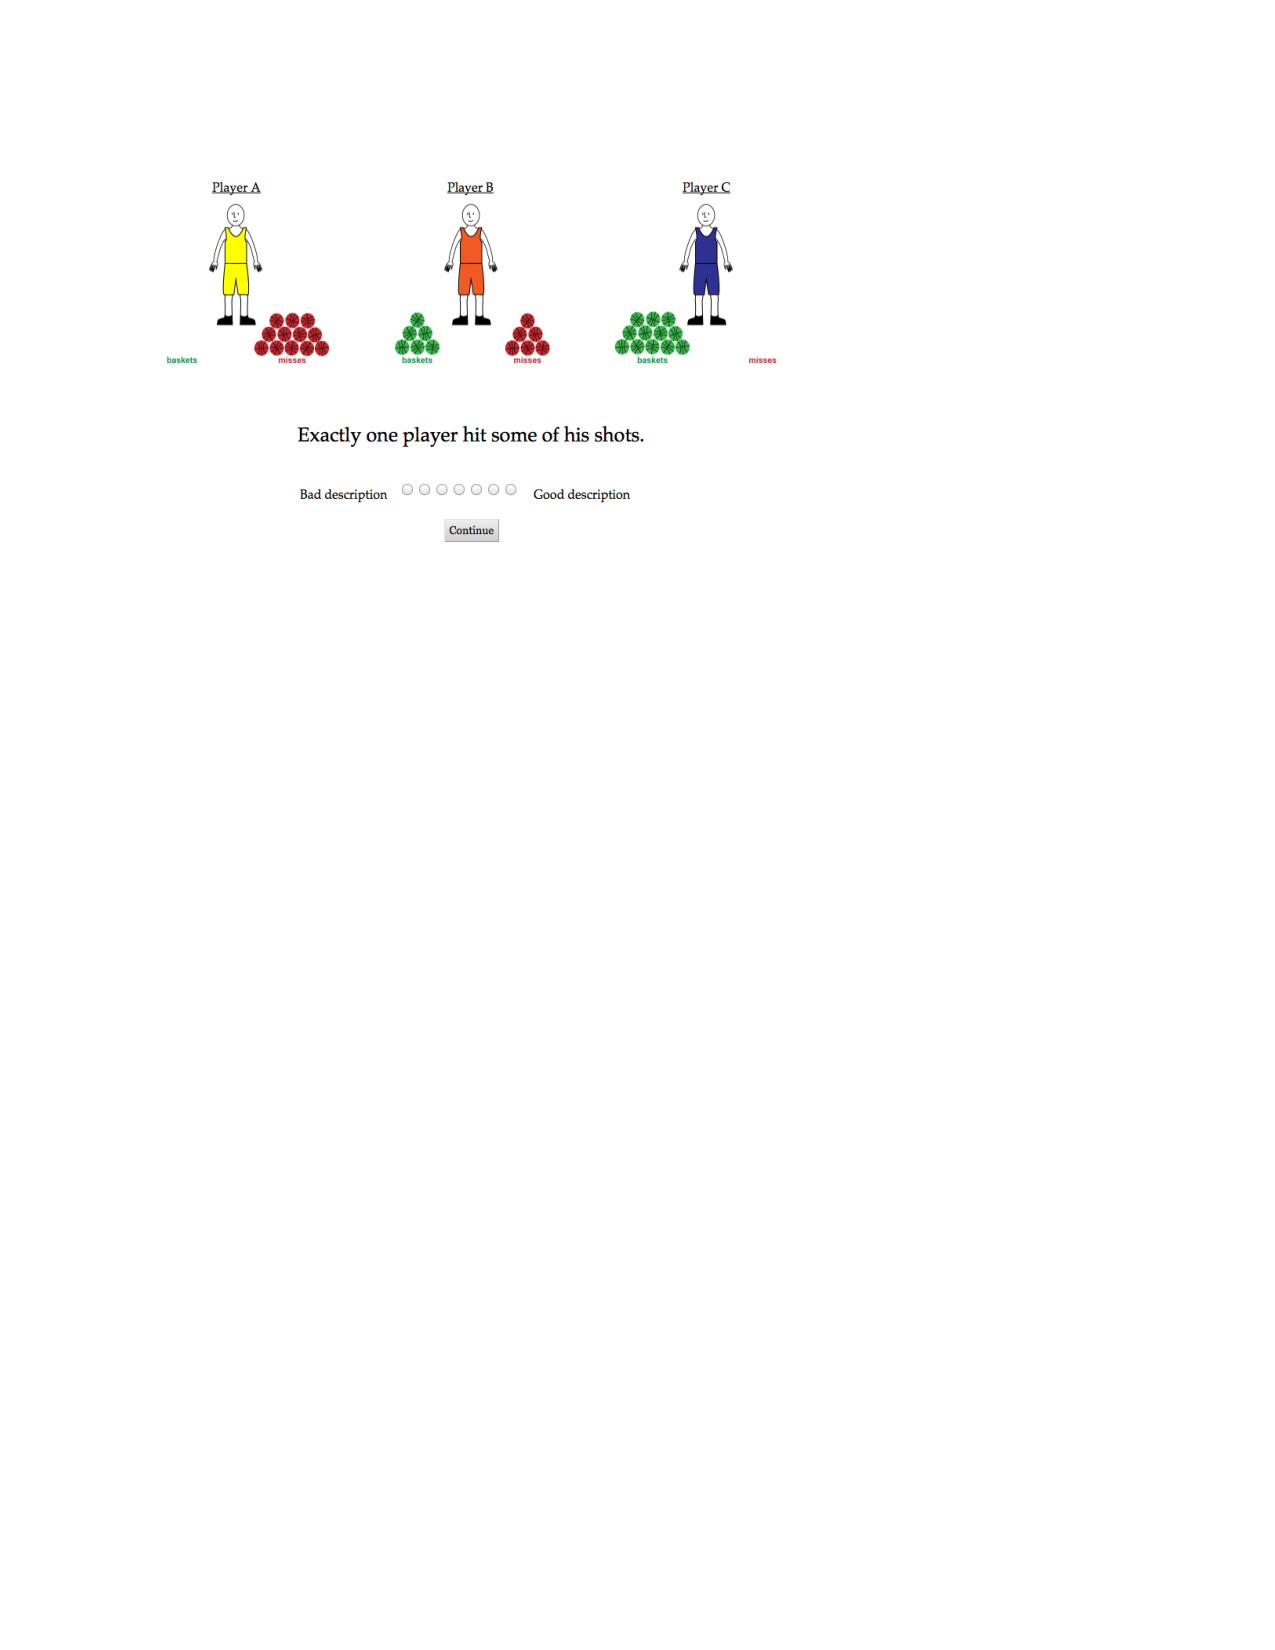
\includegraphics[scale=1]{fig/experiment-display}}
  \caption{Experiment display.}
  \label{fig:exp1}
\end{figure}

We generated displays like those in \figref{fig:exp1}. In each
display, each of the three players, A, B, and C, has taken 12
basketball shots (a number small enough for visual display but outside
of the subitizing range and thus less likely to introduce competitions
from cardinal determiners like \word{three shots};
\citealt{Degen:Tanenhaus:2014}). The shots were divided into two
piles, labeled `baskets' (green) and `misses' (red).  The colors of
the players clothes were set randomly from a palette of 14 colors.

Target sentences describing the displays were defined as follows:
%
\begin{examples}
\item\label{expmsgs} 
  $\set{
      \begin{tabular}[c]{l}
        Every \\
        Exactly one \\
        No 
      \end{tabular}}$
    player hit 
    $\set{
      \begin{tabular}[c]{l}
        all \\
        none \\
        some 
      \end{tabular}}$
    of his shots.  
\end{examples}
%
Following previous studies, we put a bound pronoun in the embedded
quantifier to try to ensure that the subject took scope over the
object. The partitive forms seem likely to further encourage
implicature calculation \citep{reed:1991-interpreting,Grodner-etal:2010,degen:inpress-SP}. We chose the verb
\word{hit} over the slightly less marked verb \word{make} to try to
avoid the sense of `make' as in `take' (consistent with missing).

For the target items, there were nine different conditions,
corresponding to the worlds in \eg{conds}, in the notation we've been
using to identify possible worlds.
%
\begin{examples}
\item\label{conds} $\set{\world{NNN}, \world{NNS}, \world{NNA},
    \world{NSS}, \world{NSA}, \world{NAA}, \world{SSS}, \world{SSA},
    \world{SAA}, \world{AAA}}$
\end{examples}
%
This is a subset of the full cross-product of the three outcomes
\world{N}, \world{S}, and \world{A} in which player $i$ always did at
least as well as player $i+1$, going left to right.  Our target
sentences were all quantified, so we don't care about the outcome for
any single player, meaning that we don't distinguish, e.g.,
\world{NNS} from \world{NSN}, allowing us to work with this smaller
set of conditions. In the experiment, the `order' of each world was
randomized, so that, e.g., \world{NSA} appeared visually in each of
its three orders approximately the same number of times.

\subsubsection{Procedure} 

After reading our consent form, participants were given the following
cover story:

\begin{quote}
  We are trying to train an automated sportscasting system to generate
  color commentary on simple competitions. We'd like you to make
  judgments about the quality of the comments it generates. We'll use
  these ratings to train our system further.
\end{quote}

After reading the cover story and some instructions, participants were
presented with three training items, designed to ensure that participants
understood the cover story, displays, and sentences. They then judged 32
sentences, divided into nine target sentences and 23 fillers. The
design was between-subjects: no experimental participant judged the same sentence twice. 
 
Each sentence received a total of 300 responses. For the target
sentences, each sentence--world pair received between 19 and 44
responses (mean 30); this variation resulted from randomization of the
assignment of worlds to sentences.

Target sentences were presented below displays. Participants were
asked to evaluate sentences on a seven-point Likert scale ranging from
`Bad description' to `Good description'. Our rationale for using this
scale is that it allows enough space for participants to both register
a truth-value assessment and convey information about the quality of
the report. (In this sense, our participants acted as listeners who
got to observe the speaker's state and assess the extent to which the
speaker succeeded in conveying that state with her utterance.)

All the materials and response data for the experiment are available at
the website for this paper.

%=====================================================================

\subsection{Results}\label{sec:exp1:results}

\Figref{fig:exp1-results} summarizes the responses by target sentence
and the world in which it was evaluated. Overall, participants made
judgments that accurately reflected whether sentences were true or
false; accuracy was especially clear for the sentences in the first
two columns, which do not admit pragmatic enrichment. For these cases,
the average ratings are very close to 1 (the lowest
value) where the sentence is false, and the ratings average above 6
(the second highest value) where the sentence is true. The pattern of
judgments in these conditions thus suggests that our method is
appropriate for measuring participants' interpretations.\footnote{The
  only exception to this general pattern is the sentence \word{No
    player hit none of his shots} (bottom middle), which received
  lower than normal ratings in all its true conditions and relatively
  high ratings for \world{NNN}, where it is false on its literal
  construal. We hypothesize that this pattern reflects a negative
  concord construal, on which the embedded term is interpreted as
  equivalent to \word{any of his shots}, creating a meaning that is
  true only in \world{NNN}. Negative concord of this sort is
  productive in many dialects of English and understandable in all or
  nearly all of them. This likely created uncertainty about the
  intended meaning of the sentence, leading participants to disfavor
  it in general.}

\begin{figure}[!ht]
  \centering
  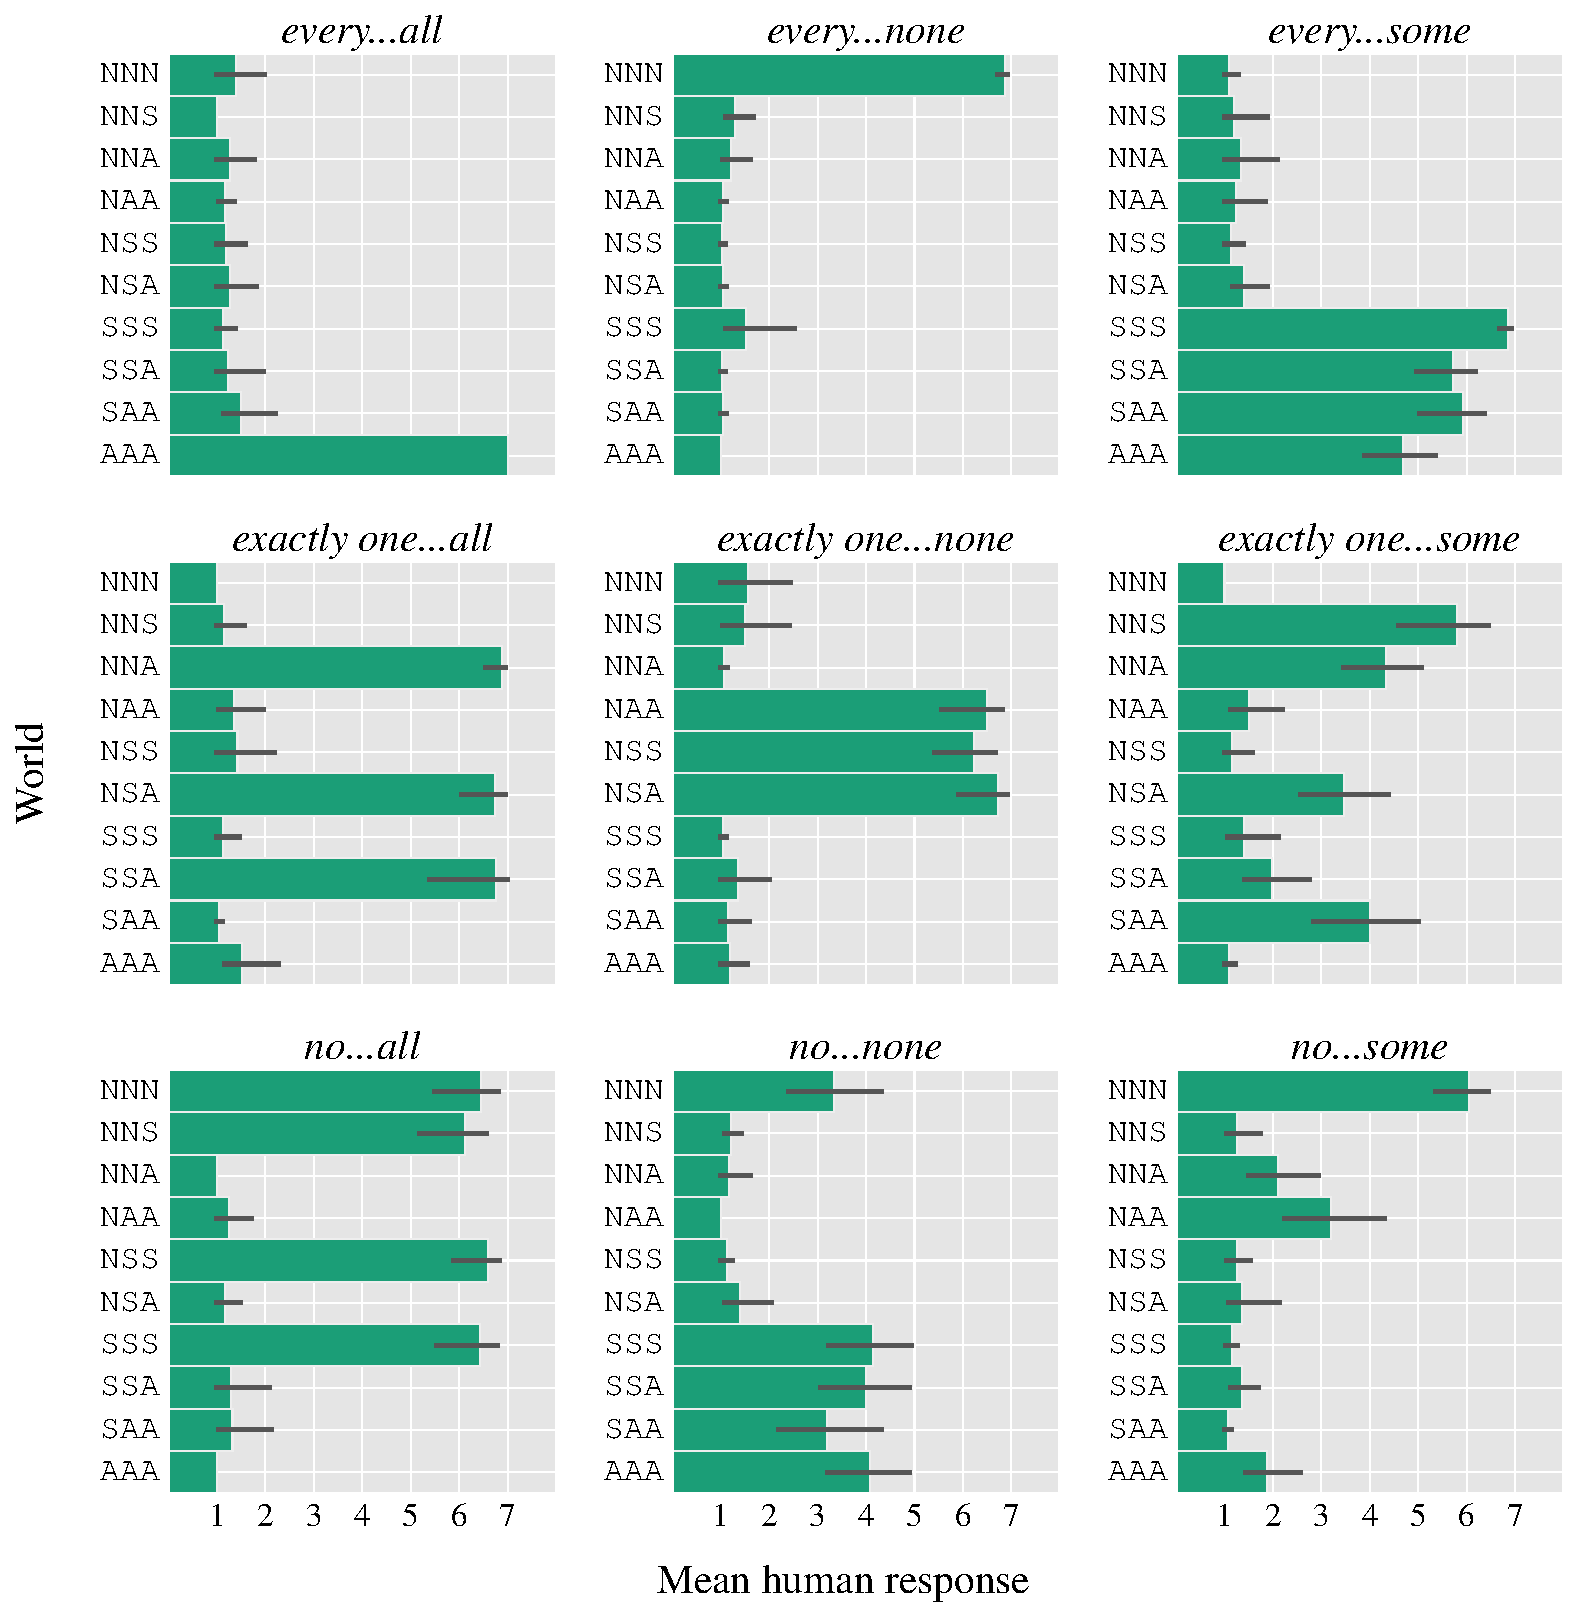
\includegraphics[width=0.85\textwidth]{fig/basketball-pilot-2-11-14-results-parsed}
  \caption{Mean ratings by sentence with bootstrapped 95\% confidence intervals.}
  \label{fig:exp1-results}
\end{figure}

We now turn to the critical conditions, reporting significance levels
for key theoretical comparisons based on the nonparametric
Mann-Whitney U test. Responses for \target{every}{some} (upper right)
were consistent with the hypothesis that \emph{some} is locally
enriched in this condition. In particular, this sentence received its
highest ratings in the \world{SSS} world. As we reviewed in
\secref{sec:implicature}, example \eg{everysome-sem}, in order to
count as a complete report in this world, this sentence requires
either local enrichment or a Gricean calculation with auxiliary
premises. Worlds \world{SSA} and \world{SAA} received the next highest
ratings (lower than \world{SSS}; both at $p<0.001$), and of all the
literally true worlds for this condition world \world{AAA} received
the lowest rating (lower than \world{SSA} and \world{SAA}; both at
$p<0.05$).  Only a simple Gricean calculation is required to account
for the higher rating of \world{SSA} and \world{SAA} compared with
\world{AAA}: in the latter world, the salient alternative \word{every
  player hit all of his shots} is a more complete description.

Nevertheless, \target{every}{some} is not a strong test of the
presence of local readings, since the entailment relations between the
readings introduce some indeterminacy into the analysis. In
particular, since the local enrichment entails the literal reading, we
can't be sure whether the high ratings for \world{SSS} derive entirely
from the availability of a local enrichment: a literal construal would
suffice to make the sentence true. Furthermore, as discussed in
\secref{sec:implicature} and in \citeauthor{Chemla:Spector:2011},
\target{every}{some} is of limited utility in distinguishing
theoretical proposals anyway. It is the \target{exactly one}{some}
sentence that allows us to probe most confidently for local readings.

The response pattern for the critical item \target{exactly one}{some}
is given in the middle right of \figref{fig:exp1-results}. The highest
ratings are in the \world{NNS} condition, where it is true under its
literal and local enrichment construals. However, it also received
high ratings in the \world{NSA} and \world{SAA} worlds (both higher at
$p<0.05$ than in \world{SSA}, the world yielding the highest rating
among those in which the sentence is false both literally and under
all possible enrichments), where it is true only with local enrichment
(because two players hit at least some of their baskets in these
worlds, ruling out the literal construal).  We note also that its more
strictly truth-conditional interpretation seems to be salient as well,
as it was rated highly on average in the \world{NNA} condition.

Finally, the pattern for \target{no}{some} also suggests a non-trivial
amount of local enrichment: though \world{NNN} received the highest
average ratings, indicating a preference for a literal construal, the
ratings for \world{NNA}, \world{NAA}, and \world{AAA} are fairly high.
(The confidence intervals are wide, but a pooled comparison of
\set{\world{NNS},\world{NSA}} with
\set{\world{NNA},\world{NAA},\world{AAA}} shows the latter set to be
significantly higher-rated; $p = 0.006$.) These are the worlds in which
no player hit only some of his shots, the local enrichment. This
finding seems consistent with the low but non-negligible rates of
local enrichment that \seccitet{Chemla:Spector:2011}{4.4.4} report for
this quantifier pair. One qualification we should add here is that our
sentence is arguably somewhat unnatural in that it places \word{some},
a positive polarity item \citep{Baker70,Israel96}, in the scope of a
negative quantifier. The binding relation between the subject and the
pronoun \word{his} in the embedded phrase should force a surface-scope
reading, but we can't rule out the possibility that participants might
have found an inverse-scope construal (`some shots are such that no
player hit them') that took the scalar term out of the scope of the
negation.

We conclude from these responses that local enrichment is possible
even in non-monotone environments, and that local enrichment might be
available in downward-monotone environments as well. However, our
concern is not only whether such readings are possible or impossible,
but rather how accurately we can predict their availability on the
basis of contextual and world knowledge.  We turn now to the task of
assessing the ability of the model in \secref{sec:model} to match both
the quantitative and qualitative patterns in our experimental data.

%=====================================================================

\subsection{Model assessment}

The pattern of data we observed is sufficiently precise and detailed
that extracting its full theoretical value requires more than
arbitrary statistical tests of simple null hypotheses --- e.g., the null
hypothesis that in the \target{exactly one}{some} condition, ratings
are the same for the worlds admitted by local enrichment as for those
excluded under both global and locally-enriched interpretations.  This
and other such null hypotheses can be rejected with high confidence.
Instead, to characterize the patterns of inference that give rise to
the observed data, we use a model-comparison approach. In particular,
we evaluate four related models that each embody different
characterizations of linguistic meaning. By comparing these models, we
can gain insights into the aspects of each that contribute to
particular patterns of predictions.

For all the models, we take as given the literal semantics described
in \tabref{tab:grammar}, as well as the following features of the
context:
%
\begin{examples}
\item\label{expmod}
  \begin{examples}
  \item $\Domain = \set{\playera, \playerb, \playerc}$
  \item $\Worlds = $ the set in \eg{conds}
  \item\label{expformulae} $\Messages =
    \setlength{\arraycolsep}{2pt}
    \set{
      Q(\word{player})(\word{hit}(S\negthinspace(\word{shot}))) :
      \begin{array}{l}        
        Q \in \set{\word{exactly one}, \word{every}, \word{no}}, \\
        S \in \set{\word{every}, \word{no}, \word{some}}
      \end{array}}$
  \item $\Costs(\nullmsg) = 5$; $\Costs(\msg) = 0$ for all $\msg \in \Messages{-}\set{\nullmsg}$  
  \item Flat state prior: $\StatePrior(w) = \StatePrior(w')$ for all $w, w' \in \Worlds$
  \item Flat lexicon prior: $\LexPrior(\Lex) = \LexPrior(\Lex')$ for all $\Lex, \Lex' \in \LexSet$
  \end{examples}
\end{examples}

The domain $\Domain$ and worlds $\Worlds$ come directly from our human
experiment. Similarly, the set of messages $\Messages$ corresponds to
\eg{expmsgs}, with some adjustments to keep the logical grammar
simple. We stipulate flat priors and even costs (other than the null
message). As noted in \secref{sec:model}, we do not have empirical
estimates for these values; though better fits to the human data can
be achieved by adding assumptions about them, this risks overfitting
to the particular data we have and thus overstating the true accuracy
of the models.

The models we consider are defined as follows:
%
\begin{examples}
\item 
  \begin{examples}
  \item \tech{Literal semantics}: the predicted values are the output
    of $\listenerZero$, as in \subeg{agents}{l0}, run on the messages
    defined in \subeg{expmod}{expformulae}.
  \item \tech{Fixed-lexicon pragmatics}: the predicted values are the
    output of the uncertainty listener \subeg{agents}{L}, but all the
    lexical items have only themselves as refinements, so that the
    reasoning is entirely in terms of the base lexicon in
    \tabref{tab:grammar}.
  \item \tech{Unconstrained refinement}: the inferences of the
    uncertainty listener \subeg{agents}{L} with $\Refine(\word{some})
    = \wp(\sem{\word{some}}){-}\emptyset$
  \item \tech{Neo-Gricean refinement}: as in `Unconstrained
    refinement', but with $\Refine(\word{some}) =
    \set{\sem{\word{some}}, \sem{\word{some and not all}}}$.
  \end{examples}
\end{examples}

These models represent a broad range of approaches to linguistic
meaning. The first neglects pragmatics entirely (the model includes a
contextual prior over states, but we define it as flat). The second is
a version of the rational speech acts (RSA) model of
\citet{Frank:Goodman:2012} and \citet{Goodman:Stuhlmuller:2013}. RSA
has been shown to capture a broad range of scalar implicatures, but it
is known to be limited in its ability to derive manner implicatures
and certain classes of embedded implicature
\citep{Bergen:Goodman:Levy:2012,Bergen:Levy:Goodman:2014}. The final
two models are full versions of the one we presented in
\secref{sec:model}. They represent opposite ends of the spectrum of
non-trivial refinements. We saw in connection with
\tabref{tab:subjects} and \tabref{tab:subjects-ALTstyle} that there
might be empirical value in greatly constraining the space of
refinements.

We employ three methods of comparison: Pearson's correlation
coefficient, which measures the linear correlation between the human
responses and the model predictions; Spearman's rank correlation
coefficient, which assesses how closely the human responses and model
responses are aligned in terms of the rankings they predict; and the
mean-squared error (MSE) of the model predictions as compared with the
human responses, which summarizes the distance of the predictions from
the human behavior. The use of these three measures allows us to
detect models that reproduce quantitative correspondence (Pearson
correlation), qualitative correspondence (Spearman correlation), and
absolute fit between models and data.

Our model predictions are conditional probability distributions over
states given messages, and hence constrained to be in the range
$[0,1]$ and to sum to $1$. In contrast, our human responses are Likert
values in $\set{1,2,3,4,5,6,7}$ with no constraint that they sum to
any particular value. To align these values, we rescale the human
responses: if $x^{s}$ is the $10$-dimensional vector of mean human
responses for target sentence $s$, then each $p^{s}$ is the vector of
normalized values for that sentence, defined so that
$p^{s}_{i} = (x^{S}_{i}-1)/\sum_{j=1}^{10}(x^{S}_{j}-1)$. This simply
normalizes the Likert responses into a probability distribution; we
subtract $1$ because the lowest Likert value is $1$. The one
noteworthy thing about this calculation is that, because it is done on
a per-sentence basis, it is not a simple linear rescaling, and so it
affects all of our assessment metrics when applied to multiple
sentences at once. However, we regard it as the minimal viable
linking hypothesis relating our model with our experimental data.

\begin{figure}[!t]
  \centering
  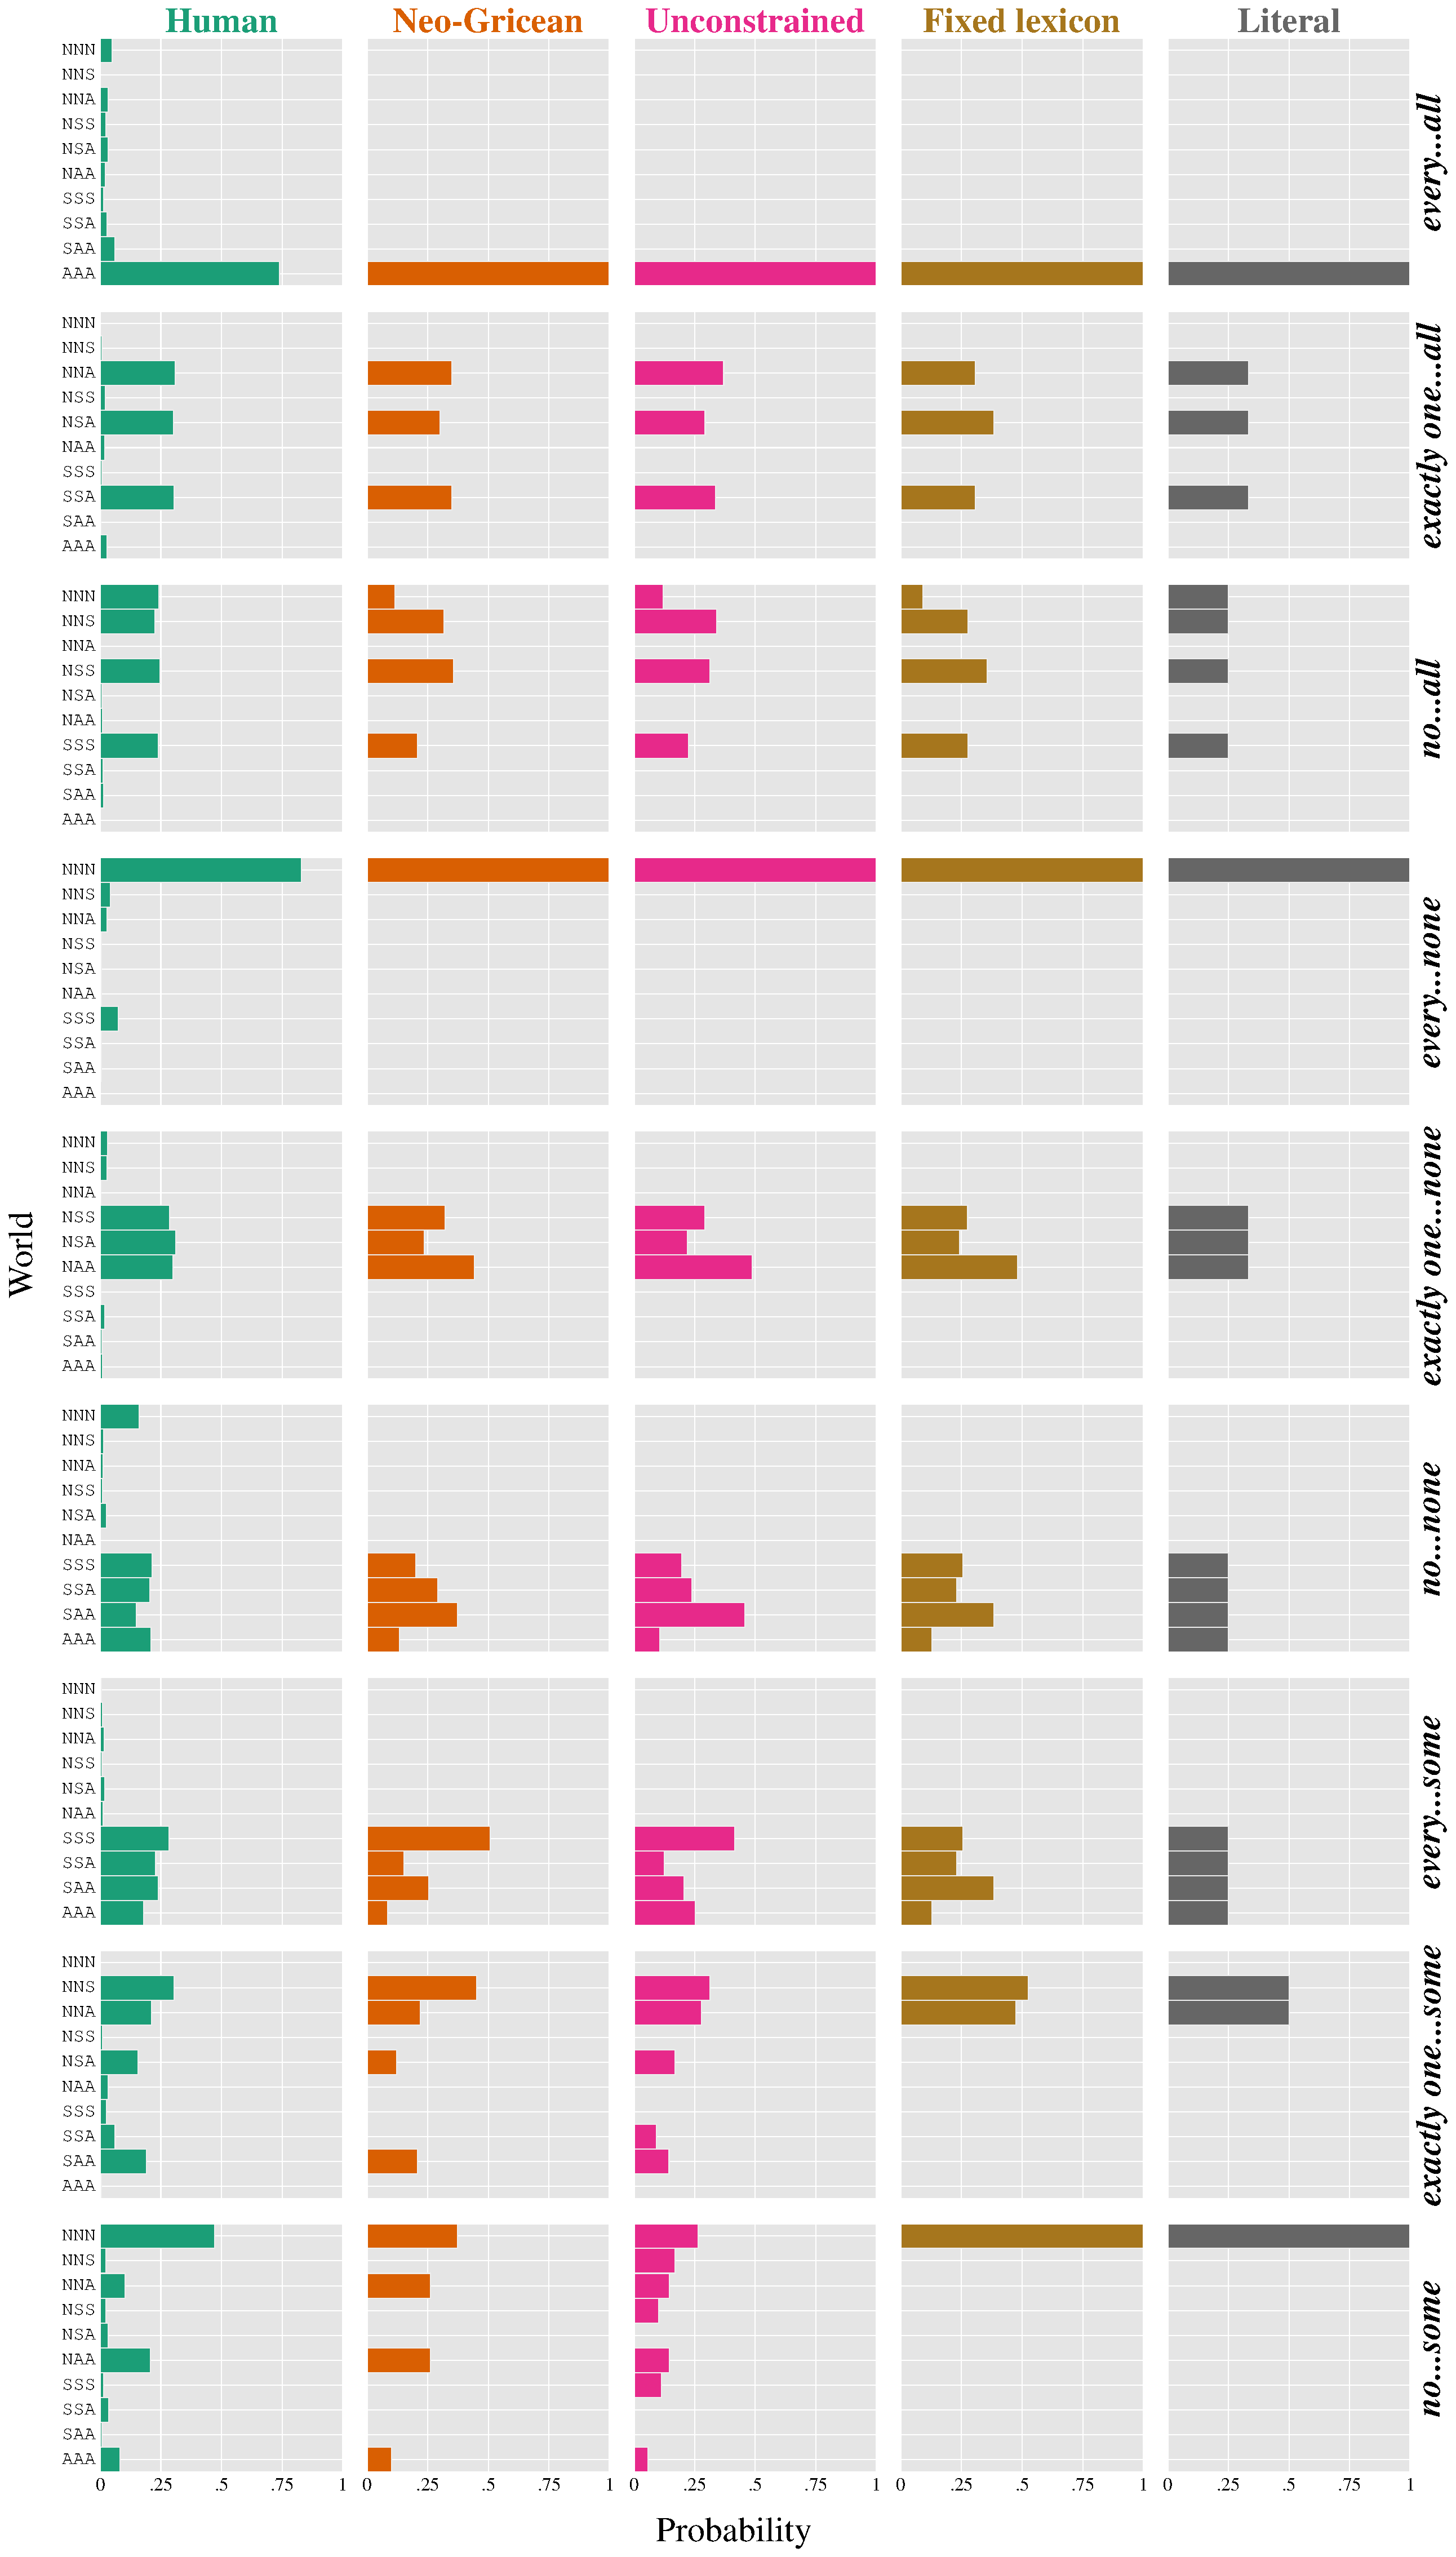
\includegraphics[height=0.92\textheight]{fig/allmodels}
  \caption{Analysis by target sentence, comparing model predictions
    with human responses.}
  \label{fig:exp-analysis}
\end{figure}

\Figref{fig:exp-analysis} summarizes the models' predictions alongside
the human responses. The predicted values are largely aligned for the
examples without \word{some} in the object position. Where \word{some}
occurs embedded, the models diverge in qualitative terms. For
\target{every}{some}, the patterns are broadly similar, but only
`Neo-Gricean uncertainty' is able to mirror the preference ordering of
responses seen in the human data. For \target{exactly one}{some}, only
the two uncertainty models are able to predict local enrichment, in
that only they assign high probability to the crucial worlds that are
false on the literal construal: \world{NSA} and \world{SAA}. The
`Literal semantics' and `Fixed-lexicon pragmatics' models are unable
to predict the salience of these construals. Similarly, only the two
uncertainty models predict \target{none}{some} to have embedded
enrichments leading to acceptability for \world{NNA}, \world{NAA}, and
\world{AAA}.

\begin{table}[!t]
  \centering
  \begin{tabular}[c]{r c c c}
    \toprule
    & Pearson & Spearman & MSE \\
    \midrule
    Literal semantics         & .94 & .76 & .0079\\
    Fixed-lexicon pragmatics  & .92 & .75 & .0094\\
    Unconstrained uncertainty & .93 & .79 & .0052\\
    Neo-Gricean uncertainty   & \graycell{.95} & \graycell{.80} & \graycell{.0046}\\
    \bottomrule   
  \end{tabular}
  \caption{Overall assessment.}
  \label{tab:overall}
\end{table}

\Tabref{tab:overall} summarizes our overall quantitative
assessment. All of the correlations are extremely high, and the MSE
values are extremely low. This is reassuring about the general utility
of all of these models for predicting human judgments. Comparing the
values is arguably more illuminating. A few patterns stand out.
First, `Fixed-lexicon pragmatics' performs the least well overall.
Since it has been shown to add substantial value in other areas of
language and cognition, we conclude that its particular approach to
enrichment is at odds with the patterns for embedded implicatures.
The precise causes are hard to pin-point, but the fact that our target
implicatures are not always enrichments of the literal content is
surely part of the problem.  Second, while `Unconstrained uncertainty'
is better than literal semantics by the Spearman and MSE metrics, it
falls behind it on the Pearson metric. We saw in connection with
\tabref{tab:subjects} that the unintuitive lexica that this model
entertains can lead to implausible final patterns. We conjecture that
this is the root cause of the model's poor performance here as well.
Third, neo-Gricean uncertainty achieves the best results across all
three of our measures. Here again, this is consistent with our
expectations based on the large illustrative example from
\secref{sec:illustrations}, where we saw that this constrained,
lexically-driven approach to choosing refinements resulted in the best
quantitative and qualitative pattern.

The overall analysis given in \tabref{tab:overall} understates the
value of both uncertainty models when it comes to the distribution of
embedded implicatures. Our target sentences provide relatively little
space for pragmatic enrichment; in \figref{fig:exp1-results}, the left
and middle columns essentially have only literal interpretations,
leaving just the right column for our pragmatic models to
shine. What's more, our qualitative review of
\figref{fig:exp-analysis} suggests that the right column examples
reveal major distinctions. It's thus worth assessing them
quantitatively in isolation. The results of such an assessment are in
\tabref{tab:crucial-items}.  The most dramatic pattern is that the two
fixed-lexicon models are unable to capture the patterns for embedded
implicatures in the non-monotone and downward monotone
environments. In contrast, both uncertainty models capture the
patterns. These tight fits are evident in \figref{fig:exp-analysis},
and it is reassuring to see them reflected in our assessment measures.

It is also striking that the literal model is competitive for
\target{every}{some}. This probably traces to the experimentally
inconvenient fact that the enriched meaning entails the literal one,
making a literal semantics a generally safe bet. It should be noted
also that the Spearman coefficient best reflects the ability of a
model to capture the preference ordering in the human data, so the
`Neo-Gricean uncertainty' model might still be the favored choice for
this case.

Finally, it seems that neither uncertainty model is clearly superior
to the other for these data.  This suggests to us that we have not yet
found precisely the right approach to refinements (alternatives). It
is tempting to try additional refinement sets to find a single model
that wins decisively for all the target examples. We are wary of doing
this because, as noted above, it runs the risk of overfitting to our
experimental responses; we could easily engineer our own success.
However, this is nonetheless a fruitful avenue for future exploration
if paired with additional experiments for further validation.

\begin{table}[t]
  \centering
  \setlength{\tabcolsep}{4pt}
  \newcommand{\rcoldiv}{\hspace{44pt}}
  
  \begin{tabular}[c]{r rrr @{\rcoldiv} rrr  @{\rcoldiv} rrr }
    \toprule
    & 
    \multicolumn{3}{c}{\target{every}{some}}{\rcoldiv} & 
    \multicolumn{3}{c}{\target{exactly one}{some}}{\rcoldiv} &
    \multicolumn{3}{c}{\target{no}{some}} \\
    & 
    P & S & MSE & 
    P & S & MSE & 
    P & S & MSE \\
    \midrule  
    Literal       & \graycell{.98} &            .85 & \graycell{.0008} &            .77 &            .70 &            .0188 & \graycell{.91} &            .52 &            .0343 \\
    Fixed-lexicon &            .93 &            .87 &            .0025 &            .79 &            .70 &            .0184 &            .91 &            .52 &            .0343 \\
    Unconstrained &            .91 &            .85 &            .0035 & \graycell{.97} & \graycell{.92} & \graycell{.0010} &            .74 &            .49 &            .0089 \\
    Neo-Gricean   &            .88 & \graycell{.89} &            .0066 &            .96 &            .89 &            .0029 &            .89 & \graycell{.88} & \graycell{.0042} \\
    \bottomrule
  \end{tabular}
  \caption{Assessment of crucial items. `P' = `Pearson'; `S' = `Spearman'.}
  \label{tab:crucial-items}
\end{table}

Our model's performance is sensitive to the space of competitor
messages, so it is worth asking how robust these findings are to
changes in this area. We have found that the basic pattern is robust
to a number of changes to the space of quantifiers.  The only
noteworthy finding we have to report in this regard is that allowing
\word{exactly one} into object position has a major impact: while
\world{SSS} remains the best-guess inference for the message
\target{every}{some} in this setting, \target{exactly one}{some} and
\target{no}{some} effectively lose their embedded implicature
readings.  This makes intuitive sense given the nature of the model:
if the speaker has the option to choose \word{exactly one of his
  shots}, and that form is equally costly, then surely her avoidance
of that form in favor of \word{some of his shots} is a signal that she
regards the local enrichment as infelicitous.

%%%%%%%%%%%%%%%%%%%%%%%%%%%%%%%%%%%%%%%%%%%%%%%%%%%%%%%%%%%%%%%%%%%%%%

\section{Conclusion}\label{sec:conclusion}

With this paper, we sought a synthesis between Gricean accounts of
pragmatic reasoning and grammar-driven ones like that of
\citet{ChierchiaFoxSpector08}. It seems to us inevitable that both
grammar and interaction will play leading roles in the final theory of
these phenomena; at some level, all participants in the debate
acknowledge this. Our achievement is to unify the crucial components
of these approaches in a single formal model that makes quantitative
predictions.

The key components of the model we develop are compositional lexical
uncertainty and recursive modeling of speaker and listener agents
\citep{Bergen:Levy:Goodman:2014}. The lexical uncertainty property is
in evidence in \citeauthor{ChierchiaFoxSpector08}'s account as well,
in the form of underspecified logical forms with context dependent
meanings. Our model has similar formal mechanisms but also offers an
account of how discourse participants reason under this persistent
linguistic uncertainty. This leads to an important conceptual point:
not all underspecification has to be resolved in order for robust
pragmatic enrichment to take place.

The recursive reasoning of our model is characteristic of both Gricean
approaches and signaling systems approaches; our model shares formal
properties of both but makes quantitative predictions of the sort that
can be correlated with human preferences in communication. There are
by now many models in the same family as ours (see, e.g.,
\citealt{CamererHo:2004,Jaeger:2011,Smith:Goodman:Frank:2013,Kao-etal:2014,Jaeger:Franke:2014}),
so further exploration is likely to yield an even more nuanced
picture.

In addition, we saw that the space of refinements (alternatives) has a
significant impact on the final predictions. It would thus be
worthwhile to further explore different notions of refinement, seeking
better fits with our own experimental patterns and then validating
those conclusions in follow-up experiments using our experimental
items, or applying the resulting models in new domains.  We have made
publicly available all the data and code associated with this paper in
an effort to encourage these new strands of theory development and
quantitative assessment.


%%%%%%%%%%%%%%%%%%%%%%%%%%%%%%%%%%%%%%%%%%%%%%%%%%%%%%%%%%%%%%%%%%%%%%

\bibliographystyle{sp}
\setlength{\bibsep}{0pt}
\bibliography{embedded-scalars-bib}

\end{document}

